%%%%% Beginning of preamble %%%%%
\documentclass[12pt]{article} 

%What kind of document (article) and what size
%Packages to load which give you useful commands
\usepackage{amssymb, amsmath, amsthm} 
\usepackage{epsfig,graphicx} 
\usepackage{caption}
\usepackage{subcaption}
\usepackage{authblk}
\usepackage{verbatim}


%Sets the margins
\textwidth = 6.5 in 
\textheight = 9 in 
\oddsidemargin = 0.0 in 
\evensidemargin = 0.0 in 
\topmargin = 0.0 in 
\headheight = 0.0 in 
\headsep = 0.0 in \parskip = 0.2in \parindent = 0.0in

\begin{document} 
\title{Detecting Communities Using Information Flow in Social Networks} 

\author[1]{David Darmon}
\author[2]{Elisa Omodei}
\author[3]{Cesar O. Flores}
\author[4]{Lu\'is F. Seoane}
\author[5]{Kevin Stadler}
\author[6]{Jody Wright}
\author[7]{Joshua Garland}
\author[8]{Nix Barnett}
\affil[1]{Department of Mathematics, University of Maryland, College Park}
\affil[2]{ISC-PIF, LaTTiCe-CNRS, \'Ecole Normale Sup\'erieure, Paris}
\affil[3]{School of Physics, Georgia Institute of Technology, Atlanta}
\affil[4]{ICREA-Complex Systems Lab, Universitat Pompeu Fabra, Barcelona}
\affil[5]{School of Philosophy, Psychology and Language Sciences, The University of Edinburgh, Edinburgh}
\affil[6]{Department of Microbiology and Immunology, University of British Columbia, Vancouver}
\affil[7]{Department of Computer Science, University of Colorado, Boulder}
\affil[8]{Department of Mathematics and Complexity Sciences Center, University of California, Davis}

\date{16 September 2013} 
\maketitle 

\abstract{Many complex networks are characterized by a community structure, i\@.e\@. the presence of groups of nodes that are more densely connected with each other than with the rest of the network. The algorithms developed to detect such communities usually consider the structural properties of the network, i\@.e\@. the static links between nodes. In the case of social networks this means considering, for example, ``friendship" links on Facebook or ``followers" on Twitter. We argue that these kinds of static links are not indicative of the real community structure underlying these networks, since users of social media usually have hundreds of connections even with people they are only acquaintances with. Moreover, users of social media typically only communicate with a subset of these connections, and form real communities only within these subsets. In this paper, we adapt standard community detection algorithms to account for this reality using recent work in information theoretic network analysis. We apply this approach to detect \emph{dynamical} / \emph{functional} communities in both synthetic and empirical networks, and determine how the composition of the communities changes over time. We find that by explicitly incorporating the observed dynamics of users in social media, we can identify communities hidden in the structural network.}

\section{Introduction}

% What is a community and why should we care? (This goes at the beginning of every community detection paper.)

% What is the problem with applying the standard (structural) approach to data from online social networks?
	% As Elisa points out, online `friendships' aren't as meaningful.
	% In these contexts, friendships are better defined in terms of the interactions of and between users.
	% How can we incorporate this viewpoint 

% What is some relevant previous work?
	% Shalizi's paper: identifies a useful method, but doesn't apply it to social data (it's used on neural data).
	% The transfer entropy paper: they identify *links*, but then don't take the next step to perform community detection.

Through the birth of social media, new communication tools (e.g., Twitter, Facebook and YouTube) are forever changing the way we perceive human interaction and social communities. From a scientific perspective, the massive datasets collected and stored by these social-networking sites are invaluable as they serve as virtual snapshots of humanity at any given point in time.  
As a result, these social-networking sites  (e.g., Facebook and Twitter) have not only given rise to important scientific questions which still have yet to be solved, but offer a %
%We enjoy a more democratized
%and distributed environment were everything is recorded and huge databases--snapshots of 
%humankind--are available in an amount without precedents. 
%
%As a direct consquence these social media websites (e.g., Facebook and Twitter) constitute
 perfect laboratory to study these questions as they arise.
%For us, Twitter is a first choice because data is permanently available to the
%public.)


The natural structure of these social-networking sites lends itself very nicely to the tools and framework developed by the field of network theory. 
%Furthermore, since these social media services naturally store users in groups known as ``social networks", the subfield of complex systems known as network theory provides many great tools for analyzing and investigating these snapshots of mankind. 
%One major advantage of these social media services is that 
%These web services 
%aggregate users into so-called social networks , and tools
%derived from the science of complex networks seem very adequate to investigate such systems.
Network theory is a very young field of research largely stemming from
the mathematical theory of \emph{graphs}. In mathematics a \emph{graph} $G = (V, E)$ is defined to be a set of \emph{vertices} / \emph{nodes} $V$ as well as the connections between those vertices, known as \emph{edges} / \emph{links} $E$. Extending this formalism to a network is trivial. In particular we can view a \emph{network} simply as a graph in which the nodes are actors in a system and the edges are the relationship between them. For example, in a ``social-network" the nodes are the individuals and the edges are the relationships between those individuals. While this mathematical representation of a social network seems quite rudimentary, this representation yields rich, complex, and interesting properties of these networks. 

One such property is the existence of \emph{communities}: subsets of nodes that share many more edges between themselves than  with the rest of the network. Detecting and classifying these communities is a very active area of research in network theory.  While many methods have been devised for detecting these communities from the network's \emph{structure} itself (see \cite{fortunato2010community} for a review),  effectively detecting \emph{dynamical/functional} communities is not as well researched and this is the primary focus of this paper. There are multitudes of other interesting properties from graph theory we can use to analyze a social network (e.g., \emph{centrality}, \emph{betweenness}, \emph{average shortest path}, etc.). However we will focus on two more theoretical questions:  \emph{How does one properly define a network?} and \emph{What constitutes a community within that network?}


%    Meanwhile, complex networks science is a very young field of research largely steaming from
%graph theory. In the realm of mathematics, a graph--thus a  network--is a well defined objects
%consisting of nodes and edges connecting them; and from this definition we operate to derive
%properties of networks, as Erd\"os, Barabasi and many others did during the preceding decades
%\cite{??}(something by Erd\"os-Renyi, Barabasi, Strogatz, Watts?). Perhaps a first wake up call
%about the complexity of the field arrived when toy random networks \ref{??} (Erd\"os-Renyi) could
%not account for the heavy tails in degree distributions--and yet small world structure--and other
%properties that real networks consistently featured. Luckily enough, a next generation of scientist
%was ready to accept that challenge and new models and mechanisms--such as preferential attachment
%\cite{} (Barabasi- Albert)--were devised and the heavy tails were partly tamed. It was also a proper
%time to tackle more sophisticated question such as community detection within complex networks
%\cite{??} (?) and to characterize a series of metrics such as \emph{centrality}, \emph{betweenness},
%\emph{average shortest path}, et c.

%    Once more, all these measures look fantastic on a mathematical graph: a platonic object with
%fixed and well defined nodes and edges, potentially encoding for some actual object at some level of
%abstraction. But from time to time it is interesting to face reality again and to wonder not about
%the mathematical representation, but about the object itself; about the stuff that makes up actual
%networks. In a very subtle way this paper hovers around two core issues regarding real-world complex
%networks: \emph{What does actually make up a network?} and \emph{What constitutes a community within
%a network?}

    Regarding the first question, social networking websites such as Twitter provide us with a na\"ive approach:
%There exist users registered on Twitter --potentially with people or companies behind
%them that we refer indistinctly as users--and these profiles constitute the nodes of our networks.
each individual or company registered with Twitter is referred to as a user, these users constitute potential nodes in such a social-network, the users can then \emph{follow} each other providing a well defined \emph{structural} definition of edges between nodes. While this is quite straightforward, does this structural definition of the Twitter network truly capture the \emph{dynamic} social network that is present? For example, users tweet about everything from their political views to what they had for lunch, and they use this network to transmit and share information about current events, including anything from natural disasters to pop-culture. %So far so good. But users make profiles on a social network for different reasons, and these lead to some \emph{dynamics} happening \emph{on} the nodes: they tweet, talk about each
%other, share hyperlinks to virtual contents, etc. 
More precisely, information flows between nodes of these networks through the edges of the network and this dynamic information transfer is completely lost by only viewing the network in a strictly structural sense. % that is managed by the activity taking place on the nodes of the network. 
%It is a natural thing to abstract ourselves from the twitting action to any other dynamics that could take
%place in any arbitrary kind of network, and then the question above takes a deeper dimension:
%\emph{Since this tweeting, or social interaction, or management of a flow of information is the
%underlying reason why the elements of the network have been put together: what is a network actually
%made of?} Surely not just the raw links that the twitter website provides us with.
This brings to light a very important question which the structure of the graph alone cannot answer. In particular, if the simple structure of the network is not enough to characterize the dynamic nature of a social-network, is there a way to use the nodes interactions and information transfer to more accurately describe the network? Furthermore, given a description of this social-network which takes into account information transfer, what do communities now look like? These are two of the major questions this work aims to begin answering. 

To this end, we weight the links between Twitter users to take into account this dynamic social structure, and in particular the information that is being transmitted between nodes. The focus of this paper is to analyze how taking into account this dynamic interaction between nodes effects the community structure of these networks. In other words, just because two users follow each other on Twitter does not mean they actually belong to the same community or ever communicate information to each other. However, if we take into account information flow on this network as well as network structure can we then correctly characterize which communities the two users truly belong to? We analyze this question both with real Twitter data as well as with a synthetic toy model described in Section \ref{sec:examples}. We find that using community detection on networks which take into account the networks dynamics deepens our understanding of the communities discovered both in the Twitter and the synthetic data.

%The second important question above allows
%us to further gauge our methods, and is indeed the primary and most explicitly sought goal of the
%present paper: we wish to perform very well at community detection. That is why we introduce a
%redefinition of \emph{what is the stuff of our network} in the first place: we argue that a deeper
%approach to the underlying constituents of a network--e.g. by weighting links through information
%flows--should yield community structures that render a better picture of the reality, as we
%consistently find out in both our twitter and synthetic data.

%[[David, I don't know that the following paragraph fits, what do you think?]]
%    As mentioned: assessing the community structure help us decide whether our redefinition of our
%networks is actually worth it. Real-world communities are entities that we can compare to more
%intuitive notions of what a community is--as we do in this text. We should we aware of the potential
%in our approach, as more and more algorithms are developed within the social networks to suggest
%\emph{users} or \emph{content of interest}. Once more abstracting ourselves, in a more general
%purpose network system, our contributions could shed some light on \emph{how networks should grow
%further}. At the same time, from a social-network-user point of view our methods could help us made
%more reliable definitions of who our friends are, or who are those actually influencing us.

    The paper is structured as follows: In Section \ref{sec:methods} the concepts of community structure
and community detection with and without information transfer are discussed. In this section we provide the rigorous mathematical foundations needed for the rest of the paper. 
In Section \ref{sec:examples} we explicitly outline our two example networks: a toy model, and a real
dataset from Twitter. The results of both the \emph{structural} and \emph{dynamical} community detection is discussed in Section \ref{sec:results}.
% where
%we compare communities derived from original \emph{structural} networks--as defined by the basic link structure of Twitter and of the toy model--with those obtained after the redefinition that
%we introduce. 
We further analyze the resulting communities and analyze structural changes in these networks over time in Section \ref{sec:discussion}. Finally we conclude and provide areas for future work in Sections \ref{sec:futurework} and \ref{sec:conclusions}.
\section{Methods}\label{sec:methods}

\subsection{Network and Dynamics}

First, we consider the most general case of a dynamics \emph{on} a \emph{structurally-static} network. We fix some notation, following \cite{kolaczyk2009statistical}. Let $G = (V, E)$ be the graph that represents the $|V|$ vertices in the network and the $|E|$ edges between them. We will consider a random field evolving in time on this network. That is, for a finite network, let $X(t, v)$ denote the random variable in some countable alphabet $\mathcal{X}_{v}$ associated with vertex $v$ at time $t$. Overall, $X(t, v)$ is a time-varying random field whose dynamics take place on $G$ and are affected by the topology of $G$. Thus, for fixed $t$, $X(t, \cdot)$ is a random field and for fixed $v$, $X(\cdot, v)$ is a stochastic process. We will occasionally refer to the random field at a fixed timepoint $t$ as $\mathbf{X}(t) = (X(t, v_{1}), \ldots, X(t, v_{|V|})).$

For the real world problem we consider in this paper, $G$ corresponds to an (explicit/structural) social network, and $X(t,v)$ corresponds to some observed behavior of an individual $v$ at time $t$. Since the empirical data consists of the tweeting behavior of users on Twitter, we will frequently fix $\mathcal{X}_{v} = \{0, 1\}$ with $X(t, v) = 1$ indicating that user $v$ tweeted at time instant $t$, and $X(t, v) = 0$ indicating that user $v$ did not tweet at time instant $t$.

\subsection{Community Structure}

Many real networks have a natural community structure, where disjoint subgroups of nodes exchange more connections within their subgroup than between subgroups. Formally, we want to compute the optimal division of the network that minimizes the number of links between subgroups (also called  communities). The raw number of links across boundaries of communities does not give a good partition of the  network. For example, the community structure can be a consequence of random variations in the density of links. A more reliable approach uses the configuration model \cite{newman2001random} as a null model to assess the quality of a given network partition. Newman and Girvan \cite{newman2004finding} define the modularity as follows:
\begin{equation}
Q = \frac{1}{2m} \sum_{ij} \left( A_{ij} -
\frac{k_i k_j}{2m} \right) \delta(g_i,g_j)
\label{eq.q}
\end{equation}
where $m = \frac{1}{2} \sum_{ij} A_{ij}$ is the number of links and $g_i$
indicates the label of the community the node $i$
belongs to. Notice that maximizing the above function yields a partition that minimizes the 
expected number of links falling between different communities, i.e., when 
$\delta(g_i, g_j) = 0$. 
Modularity $Q$ takes values between 0 and 1: low modularity indicates the number of links 
between distinct communities is not significantly different from the random distribution and high 
modularity indicates there is a strong community structure.

\subsection{Community Detection}

In most networks, the communities described above are not known \emph{a priori} and must be inferred using the network structure encoded in the adjacency matrix $\textbf{A}$. Such inference methods, called \emph{community detection algorithms}, come in a wide variety of forms. One of the most popular approaches is via modularity maximization: the modularity metric (\ref{eq.q}) is treated as an objective function to be maximized~\cite{newman2004finding}. Within the class of modularity maximization-based community inference, many approaches exist for performing the maximization. In this paper, we use the algorithm developed by Blondel et al\@.~\cite{blondel2008fast}, which is found to be one of the best algorithms for community detection based on modularity 
optimization, as shown by Fortunato in his review of community detection methods~\cite{fortunato2010community}. 
The algorithm works in two phases: in the first one the modularity is optimized by allowing only local changes of communities, 
and in the second one the detected communities are aggregated in order to build a new partition of the network into communities. 
These two phases are repeated iteratively until no increase of modularity is possible.

\subsection{Edge Weighting using Dynamics}

As stated in the introduction, we wish to consider how \emph{dynamics} may be used to aid in the detection of communities. In particular, if we compute a statistic of pairwise dynamics, we can use that statistic to weight the structural edges  in the network, giving a weighted adjacency matrix $\mathbf{W}.$ The generalization of modularity-based community detection algorithms to weighted networks is straightforward, assuming the weight is non-negative and that larger values indicate greater affinity between nodes~\cite{newman2004analysis}.

The weighting scheme we use in this paper is as follows. Let $X^{u} = X(\cdot, u).$ That is, in what follows we implicitly assume the stationarity of $X(t, v)$ with respect to time\footnote{If we do not assume stationarity, the statistics we compute have meaning but are no longer estimators for the parameters we describe. See~\cite{vu2009information}.}. Denoting the joint distribution of $(X^{u}, X^{v})$ as $p(x^{u}, x^{v})$ and the associated marginals as $p(x^{u})$ and $p(x^{v})$, we then define the mutual information between two individuals in the usual way~\cite{cover2012elements} as
\begin{align}
	I[X^{u}; X^{v}] &= E\left[\log_{2} \frac{p(X^{u}, X^{v})}{p(X^{u})p(X^{v})}\right]\\
	&= \sum_{x^{u} \in \mathcal{X}^{u}, x^{v} \in \mathcal{X}^{v}} p(x^{u}, x^{v}) \log_{2} \frac{p(x^{u}, x^{v})}{p(x^{u}) p(x^{v})}.
\end{align}
The mutual information is not generally bounded on a standard interval. To allow for standardized weightings, we follow~\cite{shalizi2007discovering} and normalize the mutual information, noting that
\begin{align}
	I[X^{u}; X^{v}] = H[X^{u}] - H[X^{u} | X^{v}] \leq H[X^{u}]
\end{align}
(by the non-negativity of $H[X^{u} | X^{v}]$), and equivalently
\begin{align}
	I[X^{u}; X^{v}] = H[X^{u}] - H[X^{u} | X^{v}] \leq H[X^{v}].
\end{align}
Overall, this implies that
\begin{align}
	I[X^{u}; X^{v}] \leq \min \left\{ H[X^{u}], H[X^{v}]\right\},
\end{align}
so dividing by $\min \left\{ H[X^{u}], H[X^{v}]\right\}$ gives the normalized mutual information
\begin{align}
	I^{*}[X^{u}; X^{v}] = \frac{I[X^{u}; X^{v}]}{\min \{ H[X^{u}], H[X^{v}]\}} \label{normalized-MI}
\end{align}
which lies between 0 and 1. Thus, normalized mutual information meets the criterion necessary for the straightforward use of modularity-based community detection algorithms: it is non-negative, and values closer to 1 indicate a greater dependence in the dynamics.

Of course, in an empirical study, we do not know the information theoretic quantities associated with any two users. Instead, we must infer them from an observed time series. To do so, we use the maximum likelihood estimates for all quantities~\cite{paninski2003estimation}. In the absence a parametric model (which we do not assume here), this amounts to using the plug-in estimator for $p(x^{u}, x^{v})$ in (\ref{normalized-MI}). Assuming we observe $\{ (X(t, u), X(t, v)) \}_{t = 1}^{T}$, the plug-in estimator for $p(x^{u}, x^{v})$ is simply
\begin{align}
	\hat{p}(x^{u}, x^{v}) = \frac{\#(X(t, u) = x^{u}, X(t, v) = x^{v})}{T},
\end{align}
the proportion of times we observe a particular behavior in both individuals out of all behaviors observed. Thus, the weighted adjacency matrix $\mathbf{W}$ used as input to~\cite{blondel2008fast} has entries $W_{uv} = \hat{I}^{*}[X^{u}; X^{v}]$ when $A_{uv} = 1$ and 0 otherwise.

As observed in~\cite{paninski2003estimation}, all estimators for information theoretic quantities are biased, including the plug-in estimator. However, the bias is generally proportional to the size of the joint alphabet $\mathcal{X}^{u} \times \mathcal{X}^{v}$ and inversely proportional to the sample size $T$. Since we will typically take $\mathcal{X}^{u} = \{0, 1\}$ for all individuals $u$, $|\mathcal{X}^{u} \times \mathcal{X}^{v}| = 4$, and the bias will be small for the sample sizes we consider.

\subsection{Community Detection Across Time Snapshots}

In addition to studying the community structure of a static single network, we studied how the community structure changed across time snapshots. The rationale for this analysis is that, in real Twitter data,  the mutual information between users may vary across time, and therefore the community structure of the mutual information network may change across time. As
a specific example, this type of analysis could be used to detect the birth of trending topics in the Twitter social network.

In order to perform the analysis we used two modularity algorithms
specifically designed either for time snapshots or multiplex networks (a time varying network
can be described as a multiplex network in which each time snapshot is a multiplex layer).
These two algorithms are described on the articles published by Kawadia and Sreenivasan~\cite{kawadia2012sequential}, and Mucha et al\@.~\cite{Mucha14052010}. Both algorithms are available
online as open source packages in Python and Matlab, respectively. 

\subsubsection{Kawadia and Screenivasan algorithm}

The idea of this algorithm is to find a new community partition $P_t$ for a graph snapshot $G_t$, such that the estrangement (a distance
metric that the authors defined) between the new partition and the
previous one is smaller than $\delta$. In other words, the algorithm solves
the following constrained optimization problem:

\begin{equation}
\begin{array}{l}
\operatorname*{maximize}_{P} \hfill Q(P)\\
\operatorname*{subject\, to} \hfill E(P) \le \delta,
\end{array} 
\label{eq.opt}
\end{equation}
where $E(P)$ represents the estrangement between the current
and the last community partition. The authors make use of a Lagrange
multiplier to solve this problem (for more details see \cite{kawadia2012sequential}). Unfortunately, while the algorithm
worked for the synthetic data, it did not scale to the Twitter network.

\subsubsection{Mucha et al. algorithm}

This algorithm is based in optimizing a modularity definition that
includes extra terms for the existence of different network layers,
which in this case consist of different time snapshots. The new
modularity definition that the authors propose to optimize
in order to find the change of modularity across layers is:
\begin{equation}
Q_{\text{multilayer}} = \frac{1}{2\mu} 
\sum_{ijsr} \left\{ \underbrace{ \left( 
A_{ijs}
 - \gamma_s \frac{k_{is} k_{js}}{2m_s}\right) \delta_{sr} 
 }_{\text{within layer contribution}}
 + \underbrace{\delta_{ij} C_{jsr}}_{\text{between layer contr.}}
 \right\} \delta(g_{is},g_{jr}),
\label{eq.q.layers}
\end{equation}
where $A_{ijs}$ is the element $i,j$ of the adjacency matrix of layer
$s$, $k_{is}$ the degree of node $i$ inside layer $s$, $m_s$ the
total weight of layer $s$, $g_{is}$ the community index of node $i$ inside
layer $s$. Finally, the user parameter $\gamma_s$ balances
the within layer contribution and $C_{jsr}$ balances the
between layer contribution. $C_{jsr}$ can be seen as a virtual
link between node $j$'s of two different layers $s$ and $r$. In order to optimize the modularity equation, the authors use
a generalization of the Blondel et al\@. algorithm~\cite{blondel2008fast}.

\section{Examples}\label{sec:examples}

We apply the methodology developed above to two cases: a toy model of user dynamics and a real world dataset from Twitter.

\subsection{Coupled Bernoulli Processes Embedded in a Structural Network Drawn from a Stochastic Block Model}

As a starting point, we consider a model where all of the assumptions of our method are met. In particular, a structural network exists that dictates whether or not communication may occur between nodes in the network. However, this structural network is not the sole determinant of the association between nodes in the network. Instead, behavioral association is largely determined by membership in dynamical communities, where nodes within a dynamical community tend to communicate more with each other than with nodes outside of their dynamical community. Data from this model was generated in two parts: first, the structural network was constructed, and then dynamics were simulated on the structural network, as dictated by the structural ties and the community membership's of the nodes. Details on the simulation of the structural network and the dynamical model are given in Sections \ref{Sec-SBM} and \ref{coupled-bernoulli}, respectively.

\subsubsection{Stochastic Block Model}

\label{Sec-SBM}

We use the stochastic block model~\cite{holland1983stochastic} as a generative model for the structural network. The basic stochastic block model is a popular model for simple community structure. We will specify the community of a user $u$ by $C(u)$ and the set of all communities by $\mathcal{C}$. Each individual $u$ in the network is assigned to a (latent) community $C(u) = c \in \mathcal{C}$. Edges are then placed between each user $u$ and $v$ with probability $p_{uv} = p_{C(u), C(v)}$ depending only on the membership the two users. Typically, for assortative communities, $p_{cc} > p_{cc'}$ for all $c \neq c' \in \mathcal{C}$. That is, the density of links within a community is greater than the density of links between communities, which is the standard definition of community structure. These edge probabilities can be collected into a matrix $\mathbf{P}$ where $(\mathbf{P})_{cc'} = p_{cc'}.$ If we fix $p_{cc} = p_{\text{in}}$ and $p_{cc'} = p_{\text{out}}$ for all $c \neq c' \in \mathcal{C}$, we obtain an edge probability matrix like Figure~\ref{Fig-SBM}. This clearly posses a `block' structure (hence the name ``stochastic block model'') with clear communities. The adjacency matrix for a particular realization from this model resembles Figure~\ref{Fig-SBM_Realization}.

\begin{figure}[h!]
  \centering
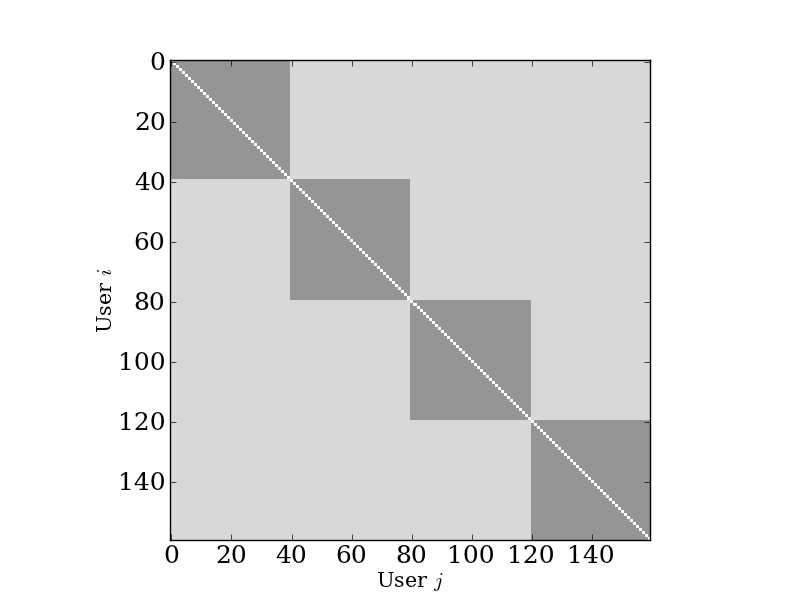
\includegraphics[width=0.75\textwidth]{Figures/prob_mat.png}
\caption{The edge probability matrix \textbf{P} for a stochastic block model with four communities each with 40 members.}
\label{Fig-SBM}
\end{figure}

\begin{figure}[h!]
  \centering
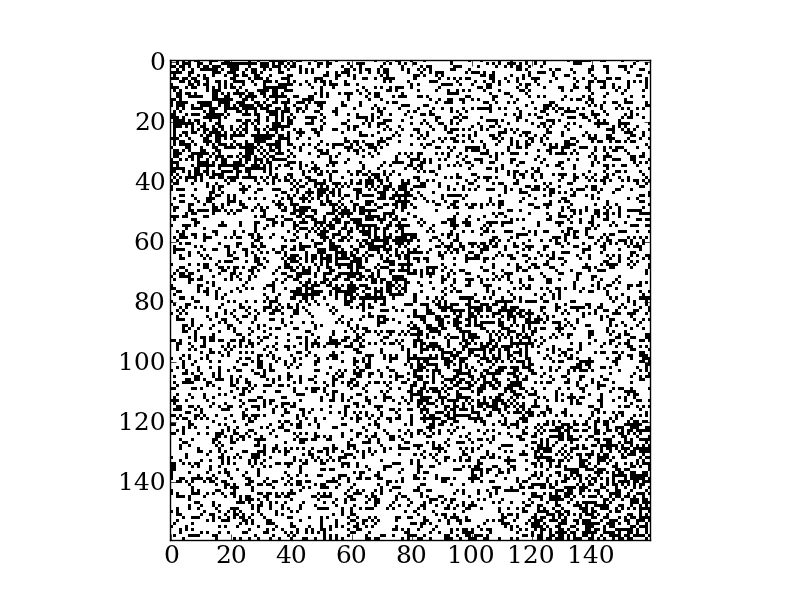
\includegraphics[width=0.75\textwidth]{Figures/adj_mat.png}
\caption{The (undirected) adjacency matrix $\mathbf{A}$ from a realization of the stochastic block model specified by the edge probability matrix \textbf{P} from Figure~\ref{Fig-SBM}.}
\label{Fig-SBM_Realization}
\end{figure}

\subsubsection{Coupled Bernoulli Process}

\label{coupled-bernoulli}

Previous work~\cite{ver2012information} has considered modeling users on Twitter as coupled Poisson processes. In this model, the users are embedded in a directed network, with each vertex in the graph corresponding to a user and each directed edge indicating the presence of `influence' of the initiating user on the terminal user. Influence was modeled as follows: after a user $u$ tweets, the user exerts an influence on its directed neighbors by increasing the instantaneous rate of their associated Poisson process for some interval of time. The authors of~\cite{ver2012information} took the coupling term to decay as a reciprocal power of the time since the tweet occurred.

In this work, we consider a modified version of this model.
\begin{comment} (\textbf{Mention connections to (directed) Susceptible-Infected-Susceptible type models?}) \end{comment}
First, since communication on digital social networks such as Twitter occurs in discrete time, we explicitly model each user as a \emph{Bernoulli} process, the discrete-time analog of a Poisson process. Second, in this initial work, we only consider an influence to occur over a single time delay. This corresponds to a choice of time scale. Thus, at a given time instant $t$, the probability of a particular user tweeting, given the entire past behavior of all of the users is
\begin{align}
	P(X(t, v) = 1 | \mathbf{X}(t-1), \mathbf{X}(t-2), \ldots) &= P(X(t,v) = 1 | \{ X(t-1, u) : u \in \mathcal{N}(v)\})\\
	&=\min \left\{p_{v} + \sum_{u \in \mathcal{N}(v)} \iota_{uv} 1[X(t-1, u) = 1], 1\right\} \label{Eq-Bernoulli_Model}
\end{align}
where $\mathcal{N}(v)$ denotes the directed neighbors of $v$ (those users in the network with directed edges from themselves to $v$), and $\iota_{uv}$ denotes the influence of user $u$ on user $v$.

\begin{figure}[h!]
  \centering
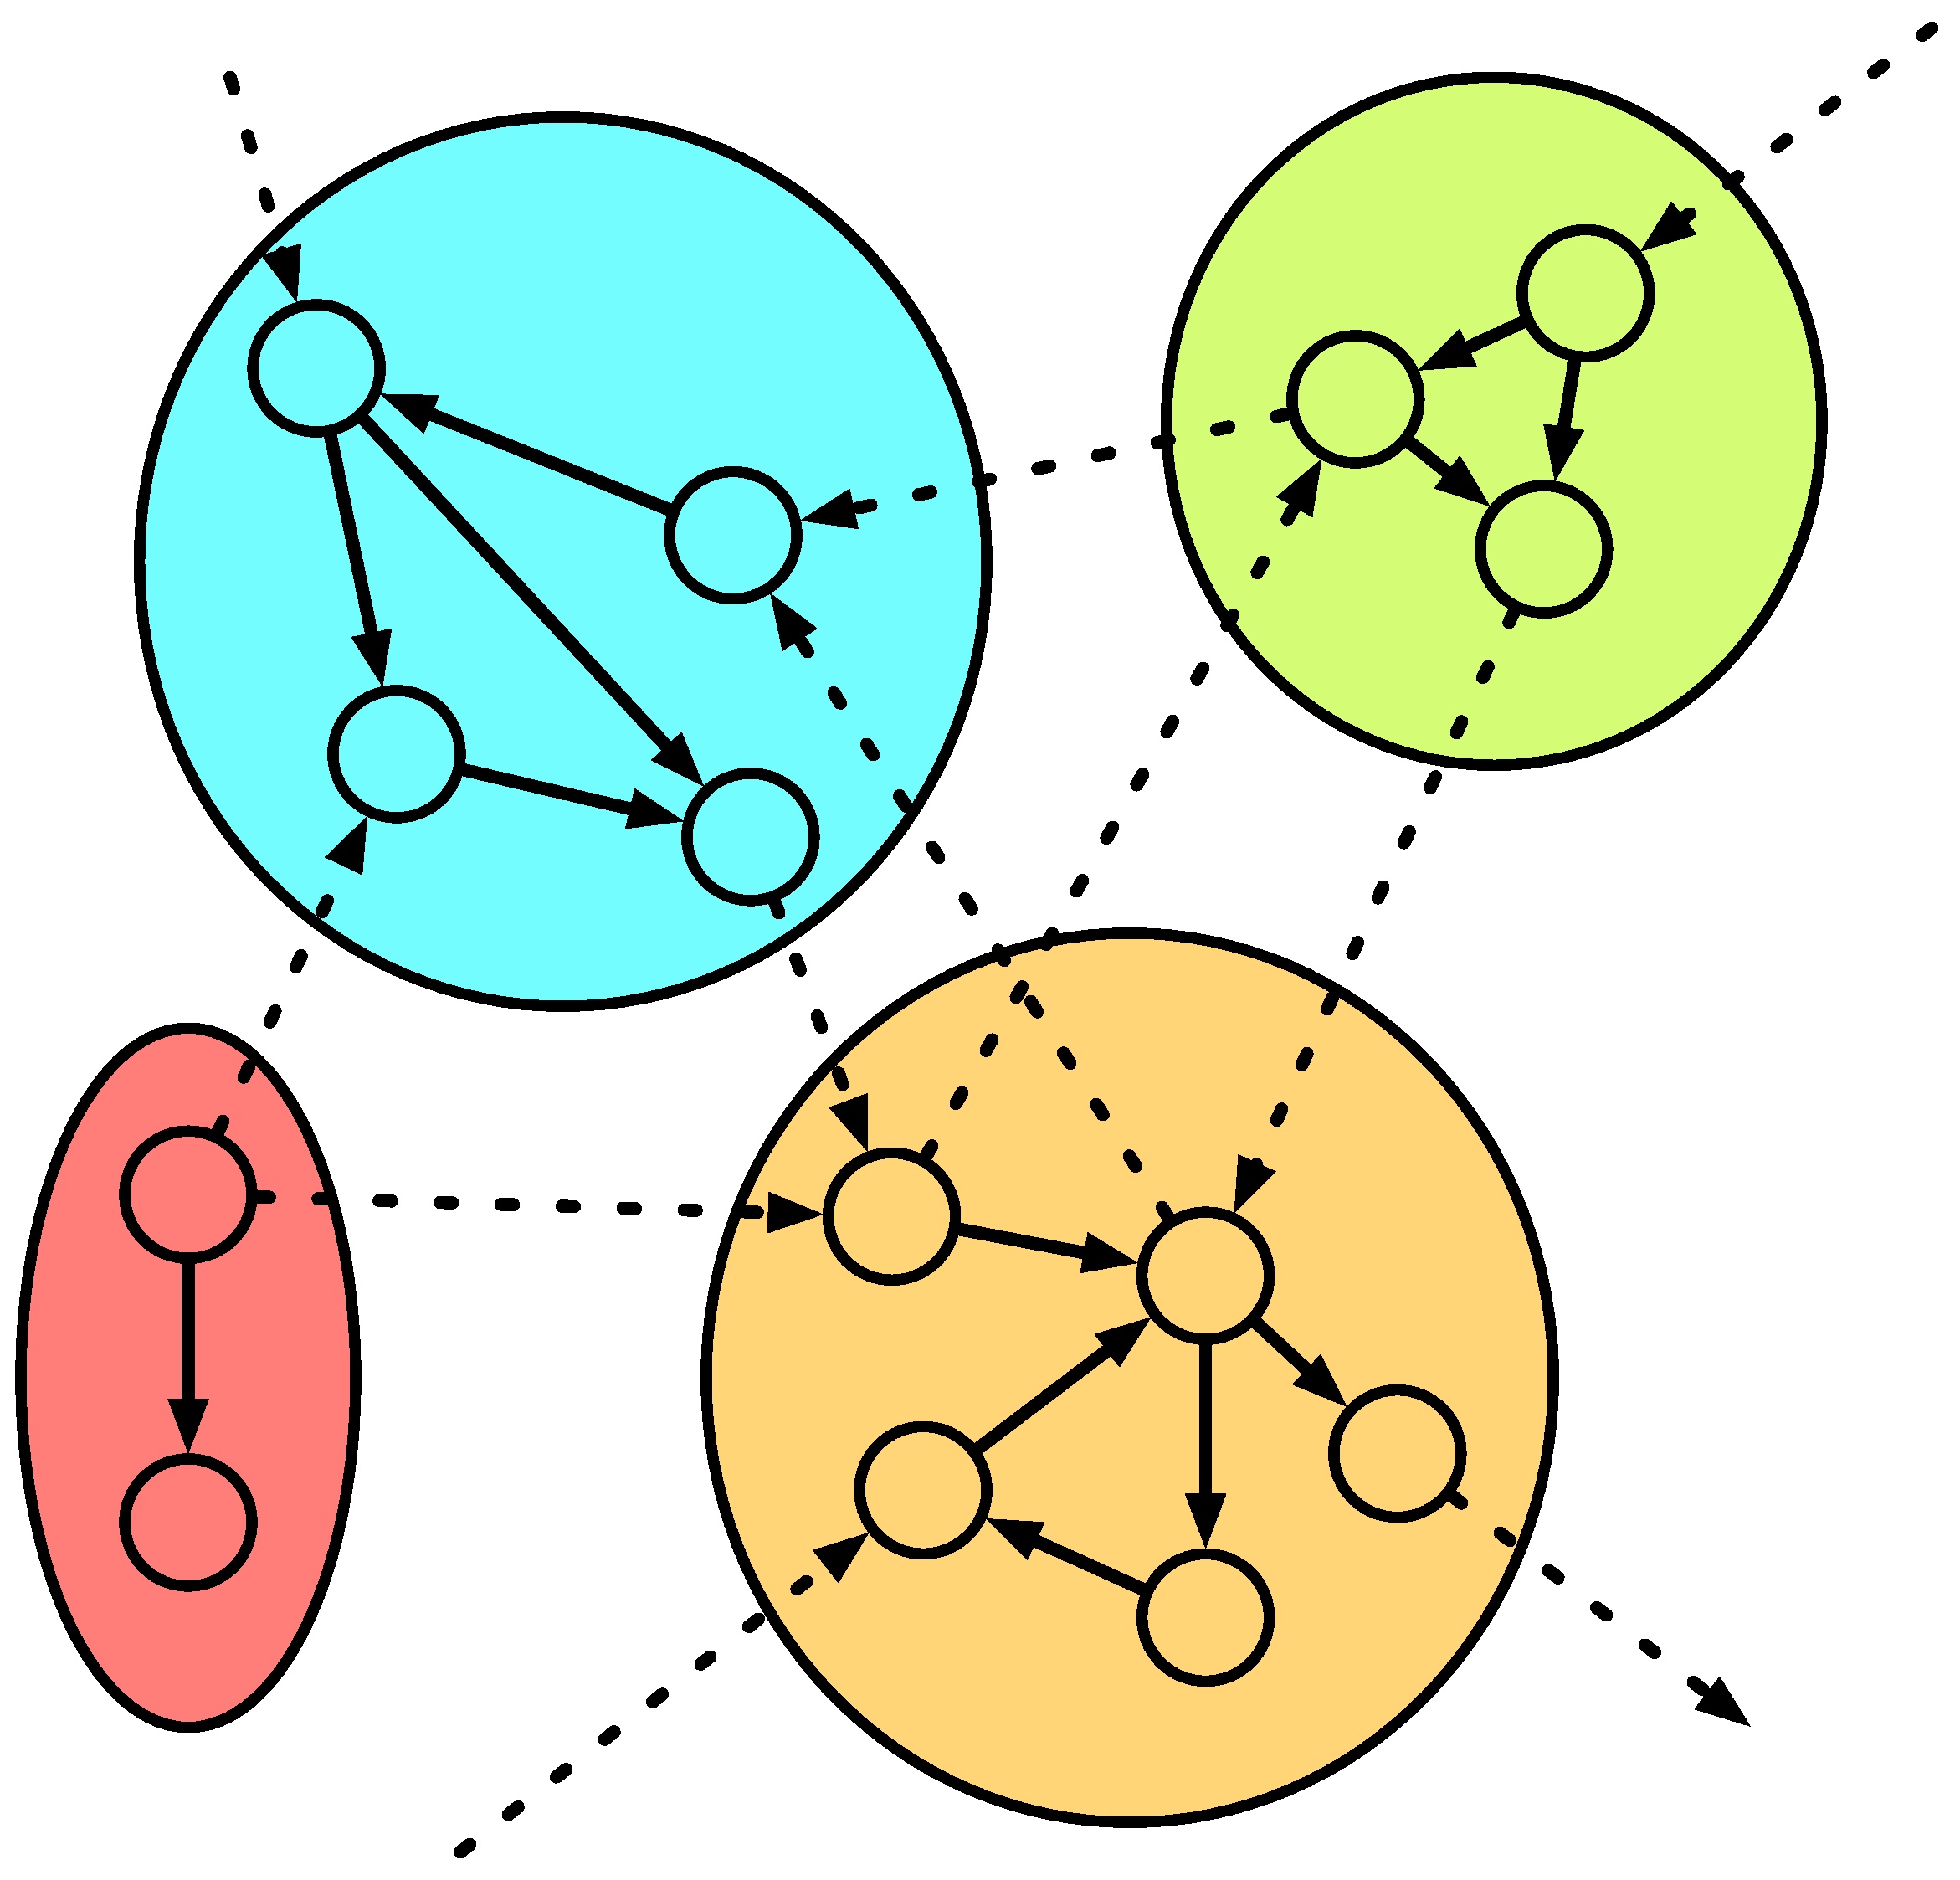
\includegraphics[width=0.3\textwidth]{Figures/Communities.eps} \hspace{1 in}
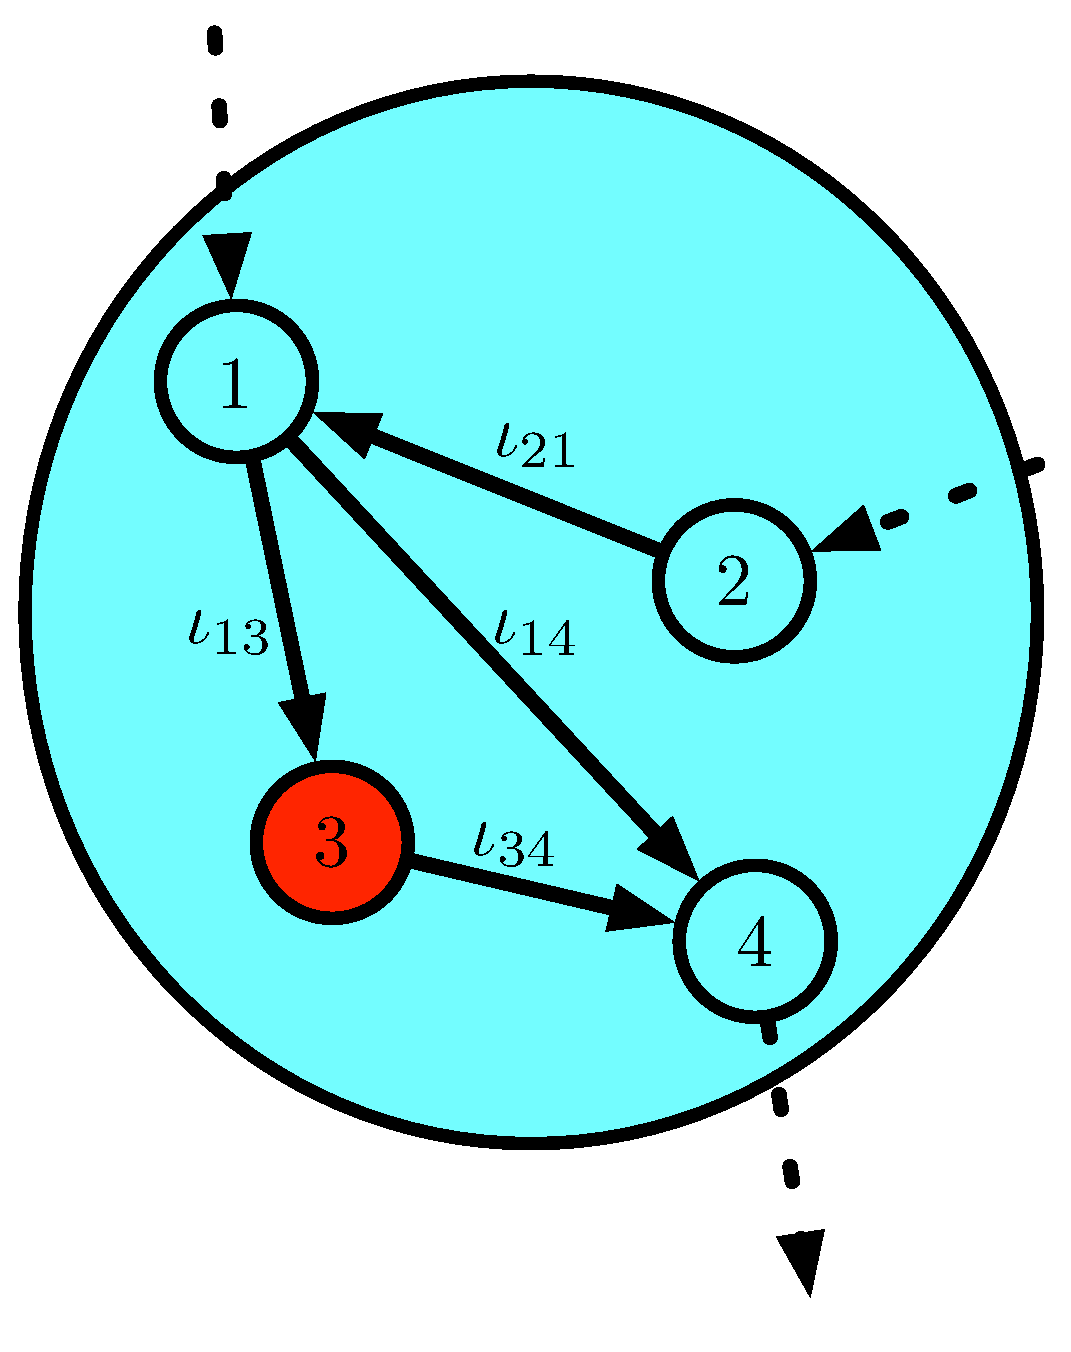
\includegraphics[width=0.3\textwidth]{Figures/Toy2.eps}
\caption{Schematics for the coupled Bernoulli model. Left: A collection of communities defined by the dynamics of their users. Right: Focusing on the influencers of a particular user.}
\label{Fig-Toy_Bernoulli}
\end{figure}

A schematic for this model is shown in Figure~\ref{Fig-Toy_Bernoulli}. In the left schematic, each solid circle corresponds to a set of nodes in a particular dynamical / functional community. Note that these communities may differ from the \emph{structural communities} as defined by the stochastic block model in Section \ref{Sec-SBM}. In particular, we will take $\iota_{uv}$ to be larger between two nodes $u$ and $v$ within the dynamical community than between two nodes in different dynamical communities. In the right schematic, we focus on user 3. For this user, we see that the equation determining the probability of that user tweeting at time $t$ (Equation (\ref{Eq-Bernoulli_Model})) reduces to
\begin{align}
	P(X(t, 3) = 1 | \mathbf{X}(t-1), \ldots) &= P(X(t,3) = 1 | X(t, 1)) \\
		&= \min \left\{p_{3} + \iota_{13} 1[X(t-1, 1) = 1], 1\right\}\\
		&= \text{base rate } + \text{ influence,}
\end{align}
a base probability plus the influence of 3's directed neighbors.

\subsubsection{Choice of Parameters for Toy Model}

For the results presented in this paper, we took $p_{\text{in}} = 0.1$ and $p_{\text{out}} = 0.05$. These values were chosen to be below the detectability threshold~\cite{decelle2011inference, mossel2012stochastic}. For values of $p_{\text{out}}$ close to $p_{\text{in}}$ (assuming that $p_{\text{in}} > p_{\text{out}}$, as would be the case for assortative social networks), community structure cannot be reliably inferred. Thus, while structural communities are present, any structural communities inferred using the structural network alone will be spurious. For each edge generated by the stochastic block model, the direction of the edge was chosen at random. We took $\iota_{\text{in}} = \frac{0.7}{4}$ and $\iota_{\text{out}} = \frac{0.07}{4}$. Thus, the influence of users within a dynamical community is ten times the influence of users outside the dynamical community. The value for $\iota_{\text{in}}$ was chosen to be below a critical value $\iota^{*}_{\text{in}}$ (dependent on $p$). Above this value, users in each community remained in a constant state of tweeting.

\subsection{Twitter Dataset}

The data consists of the Twitter statuses of 12,043 users over a 49 day period. The users are embedded in a 15,000 node network collected by performing a breadth-first expansion from a seed user. Once the seed user was chosen, the network was expanded to include his/her followers, only including users considered to be active (users who tweeted at least once per day over the past one hundred tweets). Network collection continued in this fashion by considering the active followers of the active followers of the seed, and so on.

The statuses of each user were transformed into a binary time series using their time stamp as follows. For each user $u$, we consider only the relative times of their tweets with respect to a reference time. Denote these times by $\{ \tau^{u}_{j}\}_{j = 1}^{n_{u}}$. Let the reference start time be $t_{0}$ and the coarsening amount be $\Delta t$. From the tweet times, we can generate a binary time series $\{ X(i, u)\}_{i = 1}^{T}$, where
\begin{align}
	X(i, u) = \left\{ \begin{array}{cl}
		1 &: \text{$ \exists \tau^{u}_{j} \in [t_{0} + (i - 1) \Delta t, t_{0} + i \Delta t)$} \\
		0 &: \text{ otherwise}
	\end{array}\right. .
\end{align}
In words, $X(i, u)$ is 1 if user $u$ tweeted at least once in the time interval $[t_{0} + (i - 1) \Delta t, t_{0} + i \Delta t)$, and 0 otherwise. Because the recorded time of tweets is restricted to a 1-second resolution, a natural choice for $\Delta t$ is 1 second. However, computing mutual information between second-resolution tweet series would neglect medium- to long-range influences between individuals. Thus, we generally take $\Delta t$ to be on the order of minutes.

In this paper, only tweets made between 7 AM and 10 PM (EST) were considered. For any second during this time window, a user either tweets, or does not. Thus, each day can be considered as a binary time series of length 57,600, with a 1 at a timepoint if the user tweets, and a 0 otherwise.

\section{Results}\label{sec:results}

\subsection{Community Detection --- Structural vs. Dynamical Links}

In order to test our hypothesis we used the Blondel et al\@. community detection algorithm on the two networks under analysis: the toy model and the Twitter network. 
The analysis was carried out in two steps: first we applied the algorithm to the binary unweighted network, considering in this way only the \textit{structural}
relationships between the nodes. These are given, in the case of the real data, by looking at who is \textit{following} who on Twitter, which is an
explicitly declared relationship. The limitation of this method is that most Twitter users follow a very large number of people, but in practice they
see and share only the tweets belonging to a relatively small subset of the users they follow. Therefore the second step was to apply the algorithm 
to a weighted version of the networks, that we obtained by weighting each structural link with the value of the mutual information between the two users.
The results of this analysis are shown in Table~\ref{table_modularity}.

\begin{center}
\begin{table}[!ht]
\caption{The community detection results using Blondel et al\@. without (binary) and with (weighted) normalized mutual information.}
\begin{tabular}{c|c|c|c|c|}
\cline{2-5}
& \multicolumn{2}{|c|}{Synthetic Network} & \multicolumn{2}{|c|}{Twitter Network} \\ \cline{2-5}
& Binary & Weighted & Binary & Weighted \\ \cline{1-5}
\multicolumn{1}{ |c| }{Number of Detected Communities} & 8 & 4 & 26 & 37 \\ \cline{1-5}
\multicolumn{1}{ |c| }{Optimal Modularity Value} & 0.264 & 0.625 & 0.260 & 0.404 \\ \cline{1-5}
\end{tabular}
\label{table_modularity}
\end{table}
\end{center}

We can observe a clear increase in the optimal value of modularity when we consider the weighted network, which indicates that the network has a more
defined community structure. In the case of synthetic data the value triples, whereas in the case of real data it doubles. This result shows, as we expected,
that if we weight the structural links of a network with a measure of the communication flow among the nodes, assigning more importance to the links
between two users that actually share information and less importance to the links that are there but are not exploited, we can detect a finer community structure.
In particular, for the synthetic data, we can observe that in the weighted case we find exactly four communities, which is coherent to the way
the toy model was built. A visual representation of the results is given in Figure~\ref{networks_synthetic} for the synthetic data and in 
Figure~\ref{networks_twitter} for the Twitter data.

Because the
representation of the network is different (binary vs weighted),
the modularity value is not enough to say that the community
structure is different. The differing values could be due to computing the modularity with and without weighting. To test this hypothesis, we consider the actual community structure in both cases. The sizes and overlap of the largest communities are shown in Table~\ref{Tab-Community_Stats}. By just looking at the number of communities in each representation,
we can be tempted to say that the community structure is different.
However, as Table \ref{Tab-Community_Stats} shows, the percentage of total nodes
inside the five largest communities is very high. In other words, the
 five largest communities dominate the community structure.


\begin{table}
\begin{center}
\caption{The sizes and overlaps of communities detected using the unweighted and weighted community detection algorithms.}
	\begin{tabular}{ | r | c | c | c | c | c | c |}
		\hline
		& 1 & 2 & 3 & 4 & 5 & Total \%\\ \hline
		Binary & 1092 & 941 & 410 & 292 & 12 & 97.76 \\ \hline
		Weighted & 1098 & 938 & 220 & 293 & 140 & 95.69 \\ \hline
		Shared & 876 & 777 & 66 & 244 & 0 & 69.86\label{Tab-Community_Stats} \\ \hline
		
	\end{tabular}
	\end{center}
\end{table}

First, notice that the total size (last column) of the five largest communities very high ($>95$ \%) as already described. Second, notice
that for the binary row we sorted the communities in decreasing order.
However, for the weighted row this is not the case (see community 3 and 4).
We relabel the weighted partition in order to maximize similarity
structure with the binary partition.

\begin{figure}[!ht]
\centering
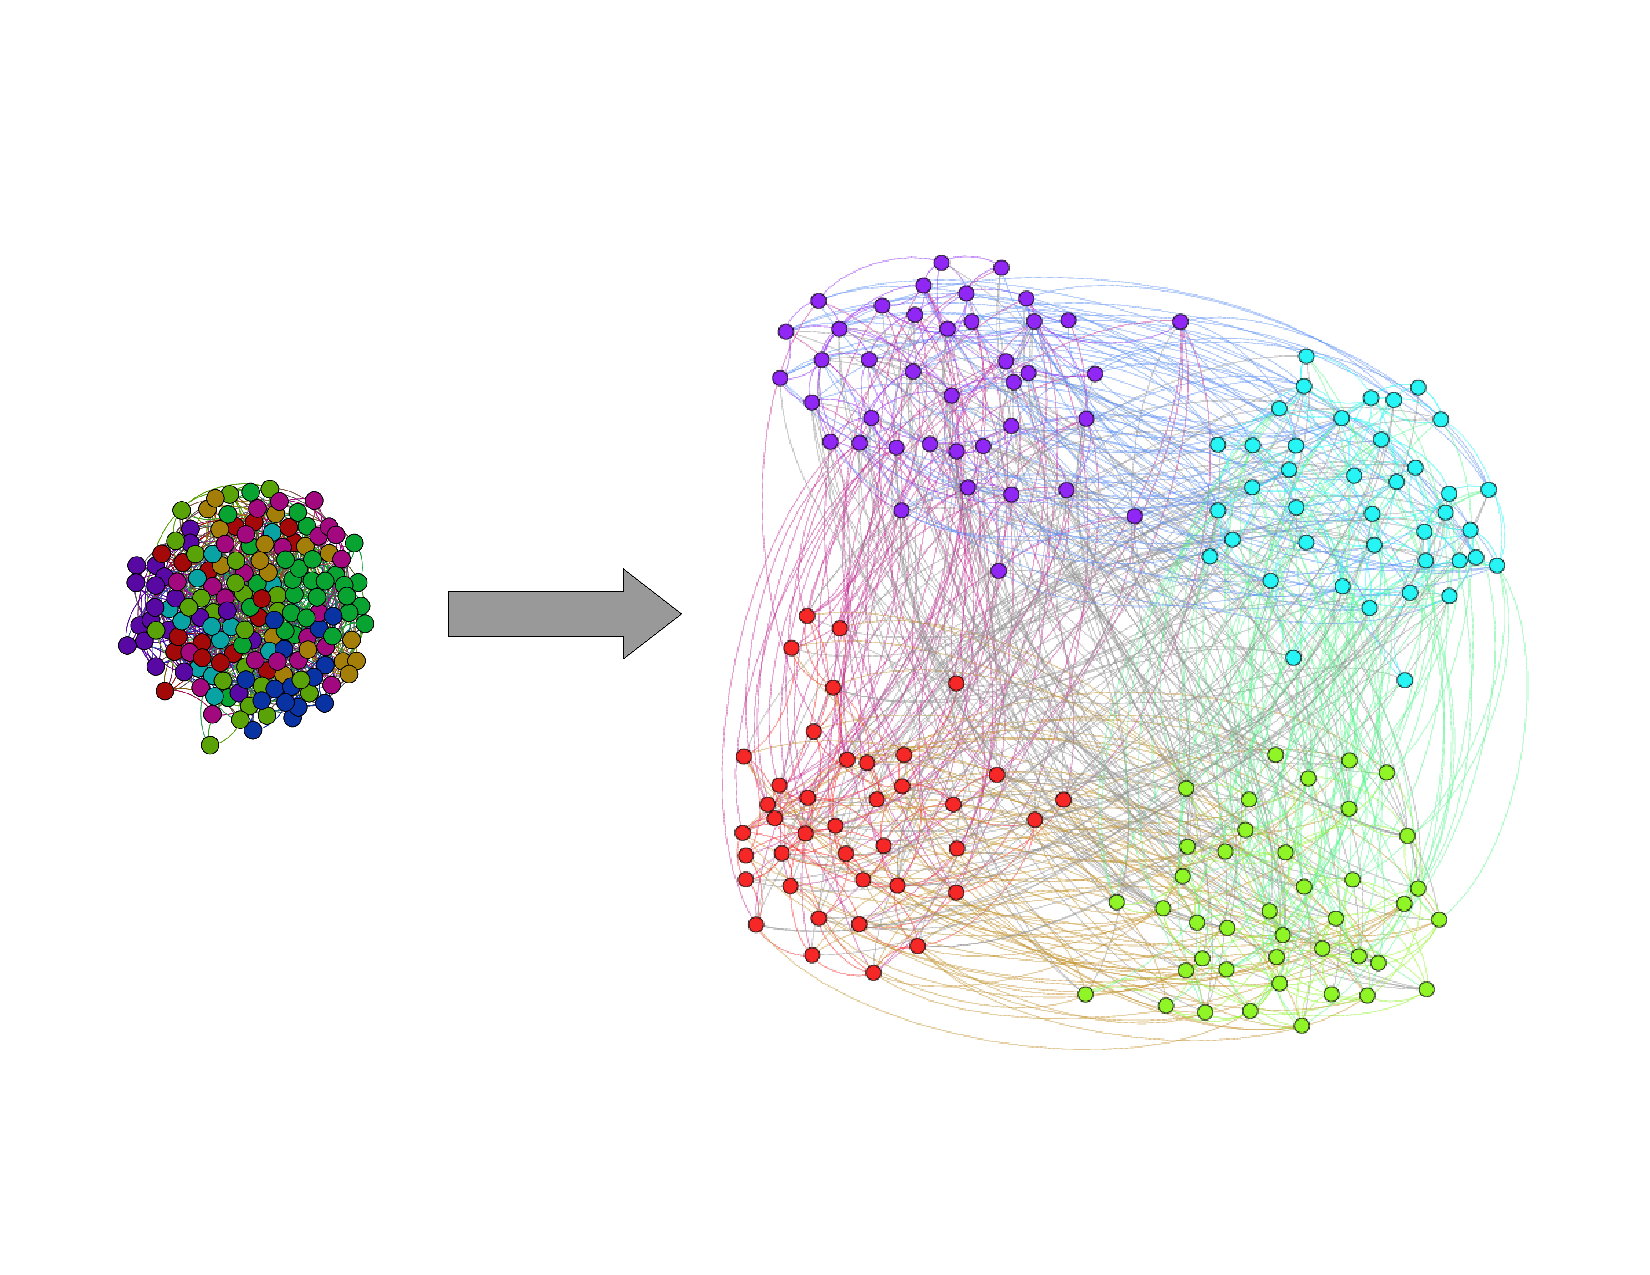
\includegraphics[width=0.72\textwidth]{Figures/synthetic_data_networks.pdf}
\caption{Visualisation of the synthetic network obtained using binary edges (left figure) and weighted ones (right figure). Node colors indicate the
community affiliation.}
\label{networks_synthetic}
\end{figure}

\begin{figure}[!ht]
\centering
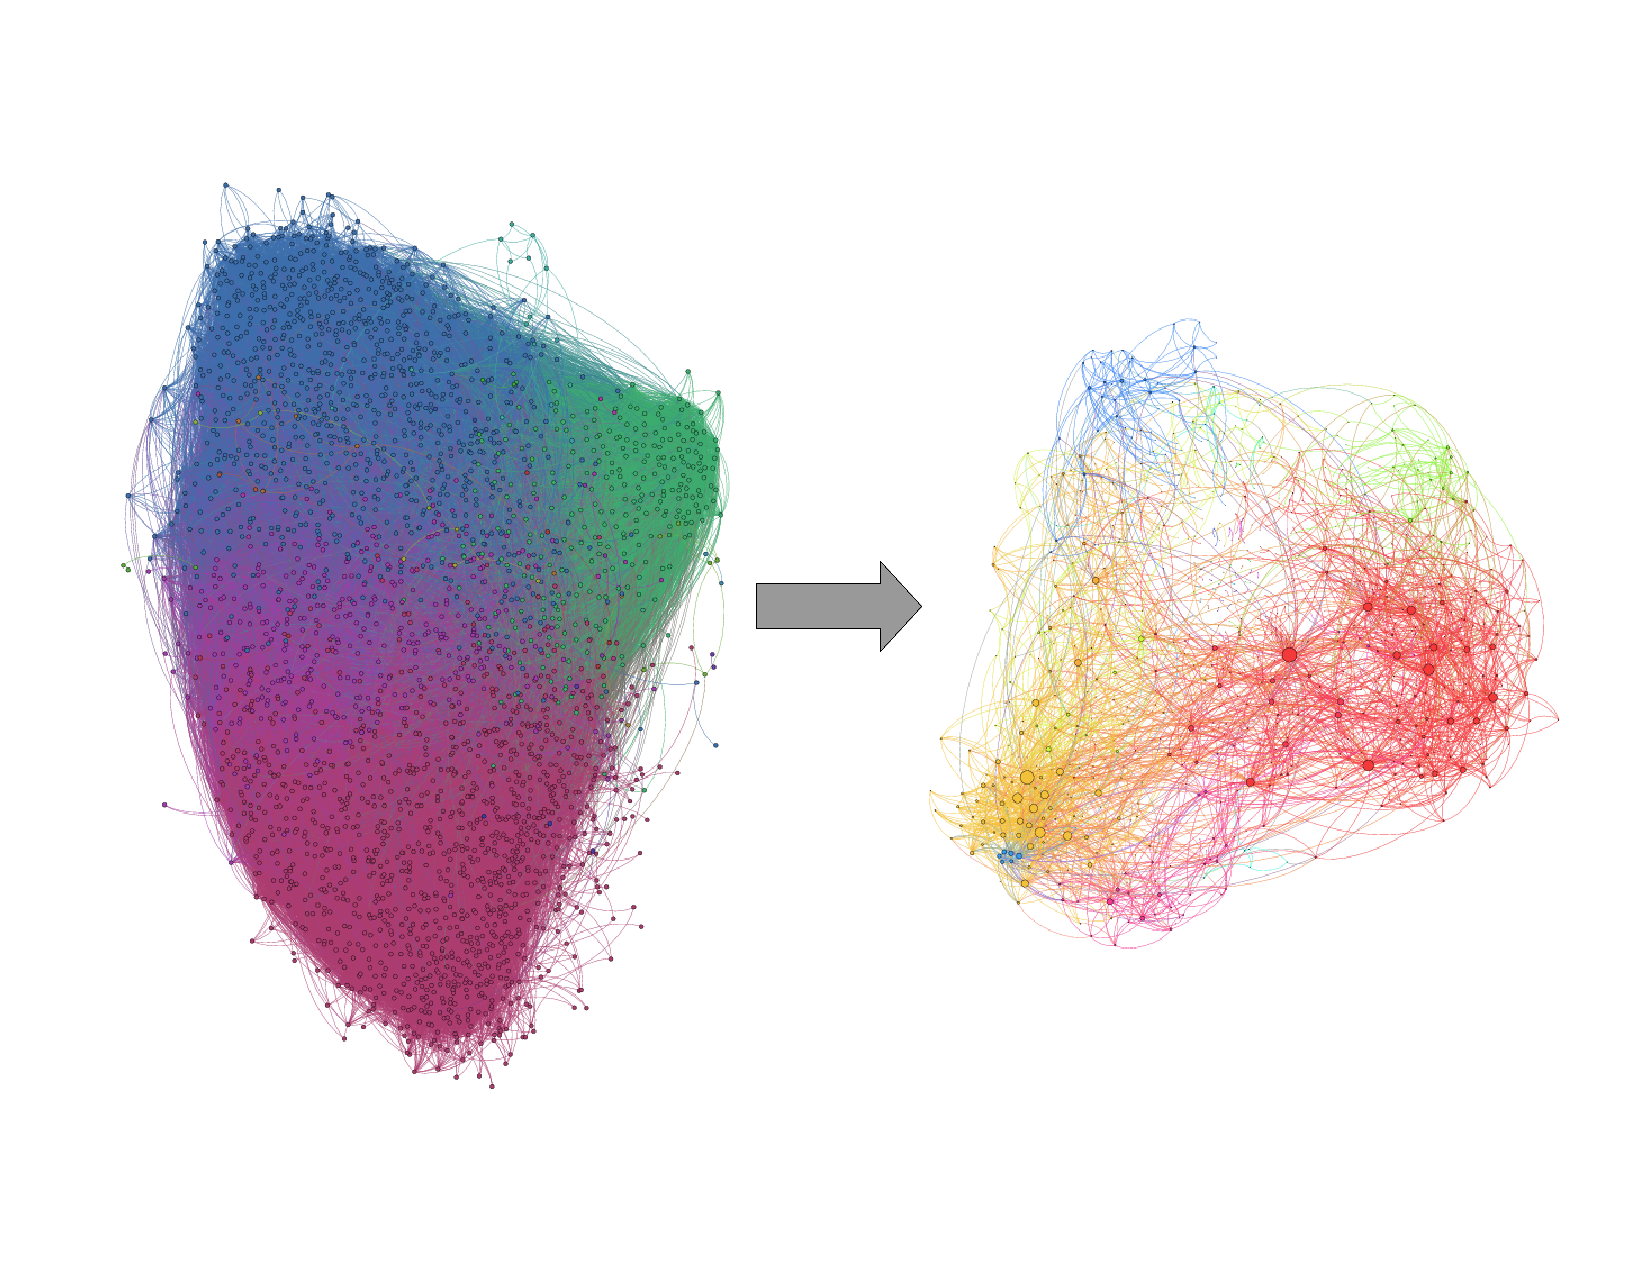
\includegraphics[width=0.72\textwidth]{Figures/twitter_data_networks.pdf}
\caption{Visualisation of the Twitter network obtained using binary edges (left figure) and weighted ones (right figure). Node colors indicate the
community affiliation.}
\label{networks_twitter}
\end{figure}

\subsection{Community Detection Across Time}

Figure \ref{fig.time.modular} represent the modularity across the
seven different weeks for a single combination of parameters. This figure shows, that in essence, the
structure does not vary across time. This fact tell us that
for this data it may be better to just evaluate the modularity
of a single snapshot across the entire seven weeks. 

\begin{figure}[!ht]
	\centering
	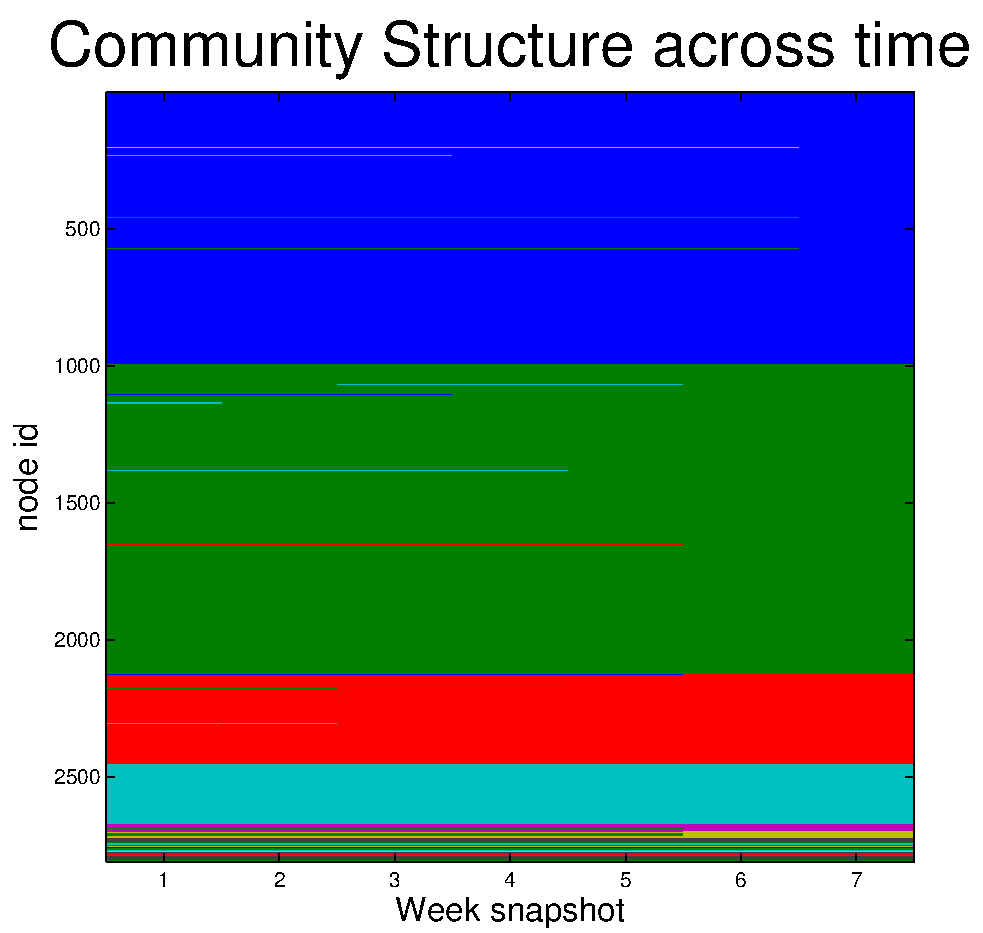
\includegraphics[width=0.87\textwidth]{Figures/modularity_time}
	\caption{Modularity across time with parameters
		$\gamma_s$ = 1 for all $s$ and $C_{jrs} = \omega=0.25$ for
		all $j,s,r$.
		 Different colors represent
		the community id to which each node (rows in this figure)
		belong to. We can observe, that the structure is dominated
		by the existence of four big communities plus a lot of small
		size communities (bottom of the Figure). Further, the modularity
		structure remains almost constant across time in the sense
		that only a very small number of nodes (represented as colored
		lines inside the big communities) switch to other communities as
		time develops.}
	\label{fig.time.modular}
\end{figure}

\section{Discussion}\label{sec:discussion}

\subsection{Comparing Structural and Dynamical Communities}

To formally compare the structural and dynamical communities, we consider the variation of information between the two community structures~\cite{meilua2003comparing}. The variation of information is defined as follows. We have two partitions $\mathcal{C} = \{C_{1}, \ldots, C_{|\mathcal{C}|}\}$ and $\mathcal{C}' = \{C'_{1}, \ldots, C'_{|\mathcal{C}'|}\}$ induced by the community structures, where the $C_{i}$ are the communities detected by each algorithm. We can compute the confusion matrix $\mathbf{N}$ from these two partitions, where
\begin{align}
	(\mathbf{N})_{kk'} = |\mathcal{C}_{k} \cap \mathcal{C}_{k'}'|.
\end{align}
From the confusion matrix, we can compute an empirical distribution over the clusters for the probability that a node randomly selected from the network belongs in community $C_{k}$ and community $C'_{k'}$,
\begin{align}
	p(k, k') = \frac{1}{|V|}(\mathbf{N})_{k k'}.
\end{align}
where we recall that $|V|$ is the number of nodes in the network. Let $X$ be the community assigned to the node by partition $\mathcal{C}$ and $Y$ be the community assigned to the node by partition $\mathcal{C}'$. The variation of information is defined in various equivalent forms as
\begin{align}
	\text{VI}[\mathcal{C}; \mathcal{C}'] &= H[X, Y] - I[X; Y] \\
	&= H[X | Y] + H[Y | X] \\
	&= H[X] + H[Y] - 2 I[X; Y],
\end{align}
or can be compactly represented in terms of the information diagram~\cite{yeung1991new} for the standard information theoretic quantities involving $X$ and $Y$ (see Figure \ref{Fig-Information_Diagram}). From the information diagram, we see that the variation of information captures the information in the joint distribution for $(X, Y)$ that is not shared. Thus, variation of information takes its maximum value when no information is shared between the two community structures, and its minimum values when the community structures are identical. It is a true metric over the space of partitions for the nodes $V$. Variation of information is bounded between 0 and $\log_{2} |V|$, and thus we will consider the normalized variation of information
\begin{align}
	\text{VI}^{*}[\mathcal{C}; \mathcal{C}'] = \frac{\text{VI}[\mathcal{C}; \mathcal{C}']}{\log_{2}|V|}.
\end{align}

\begin{figure}[h!]
  \centering
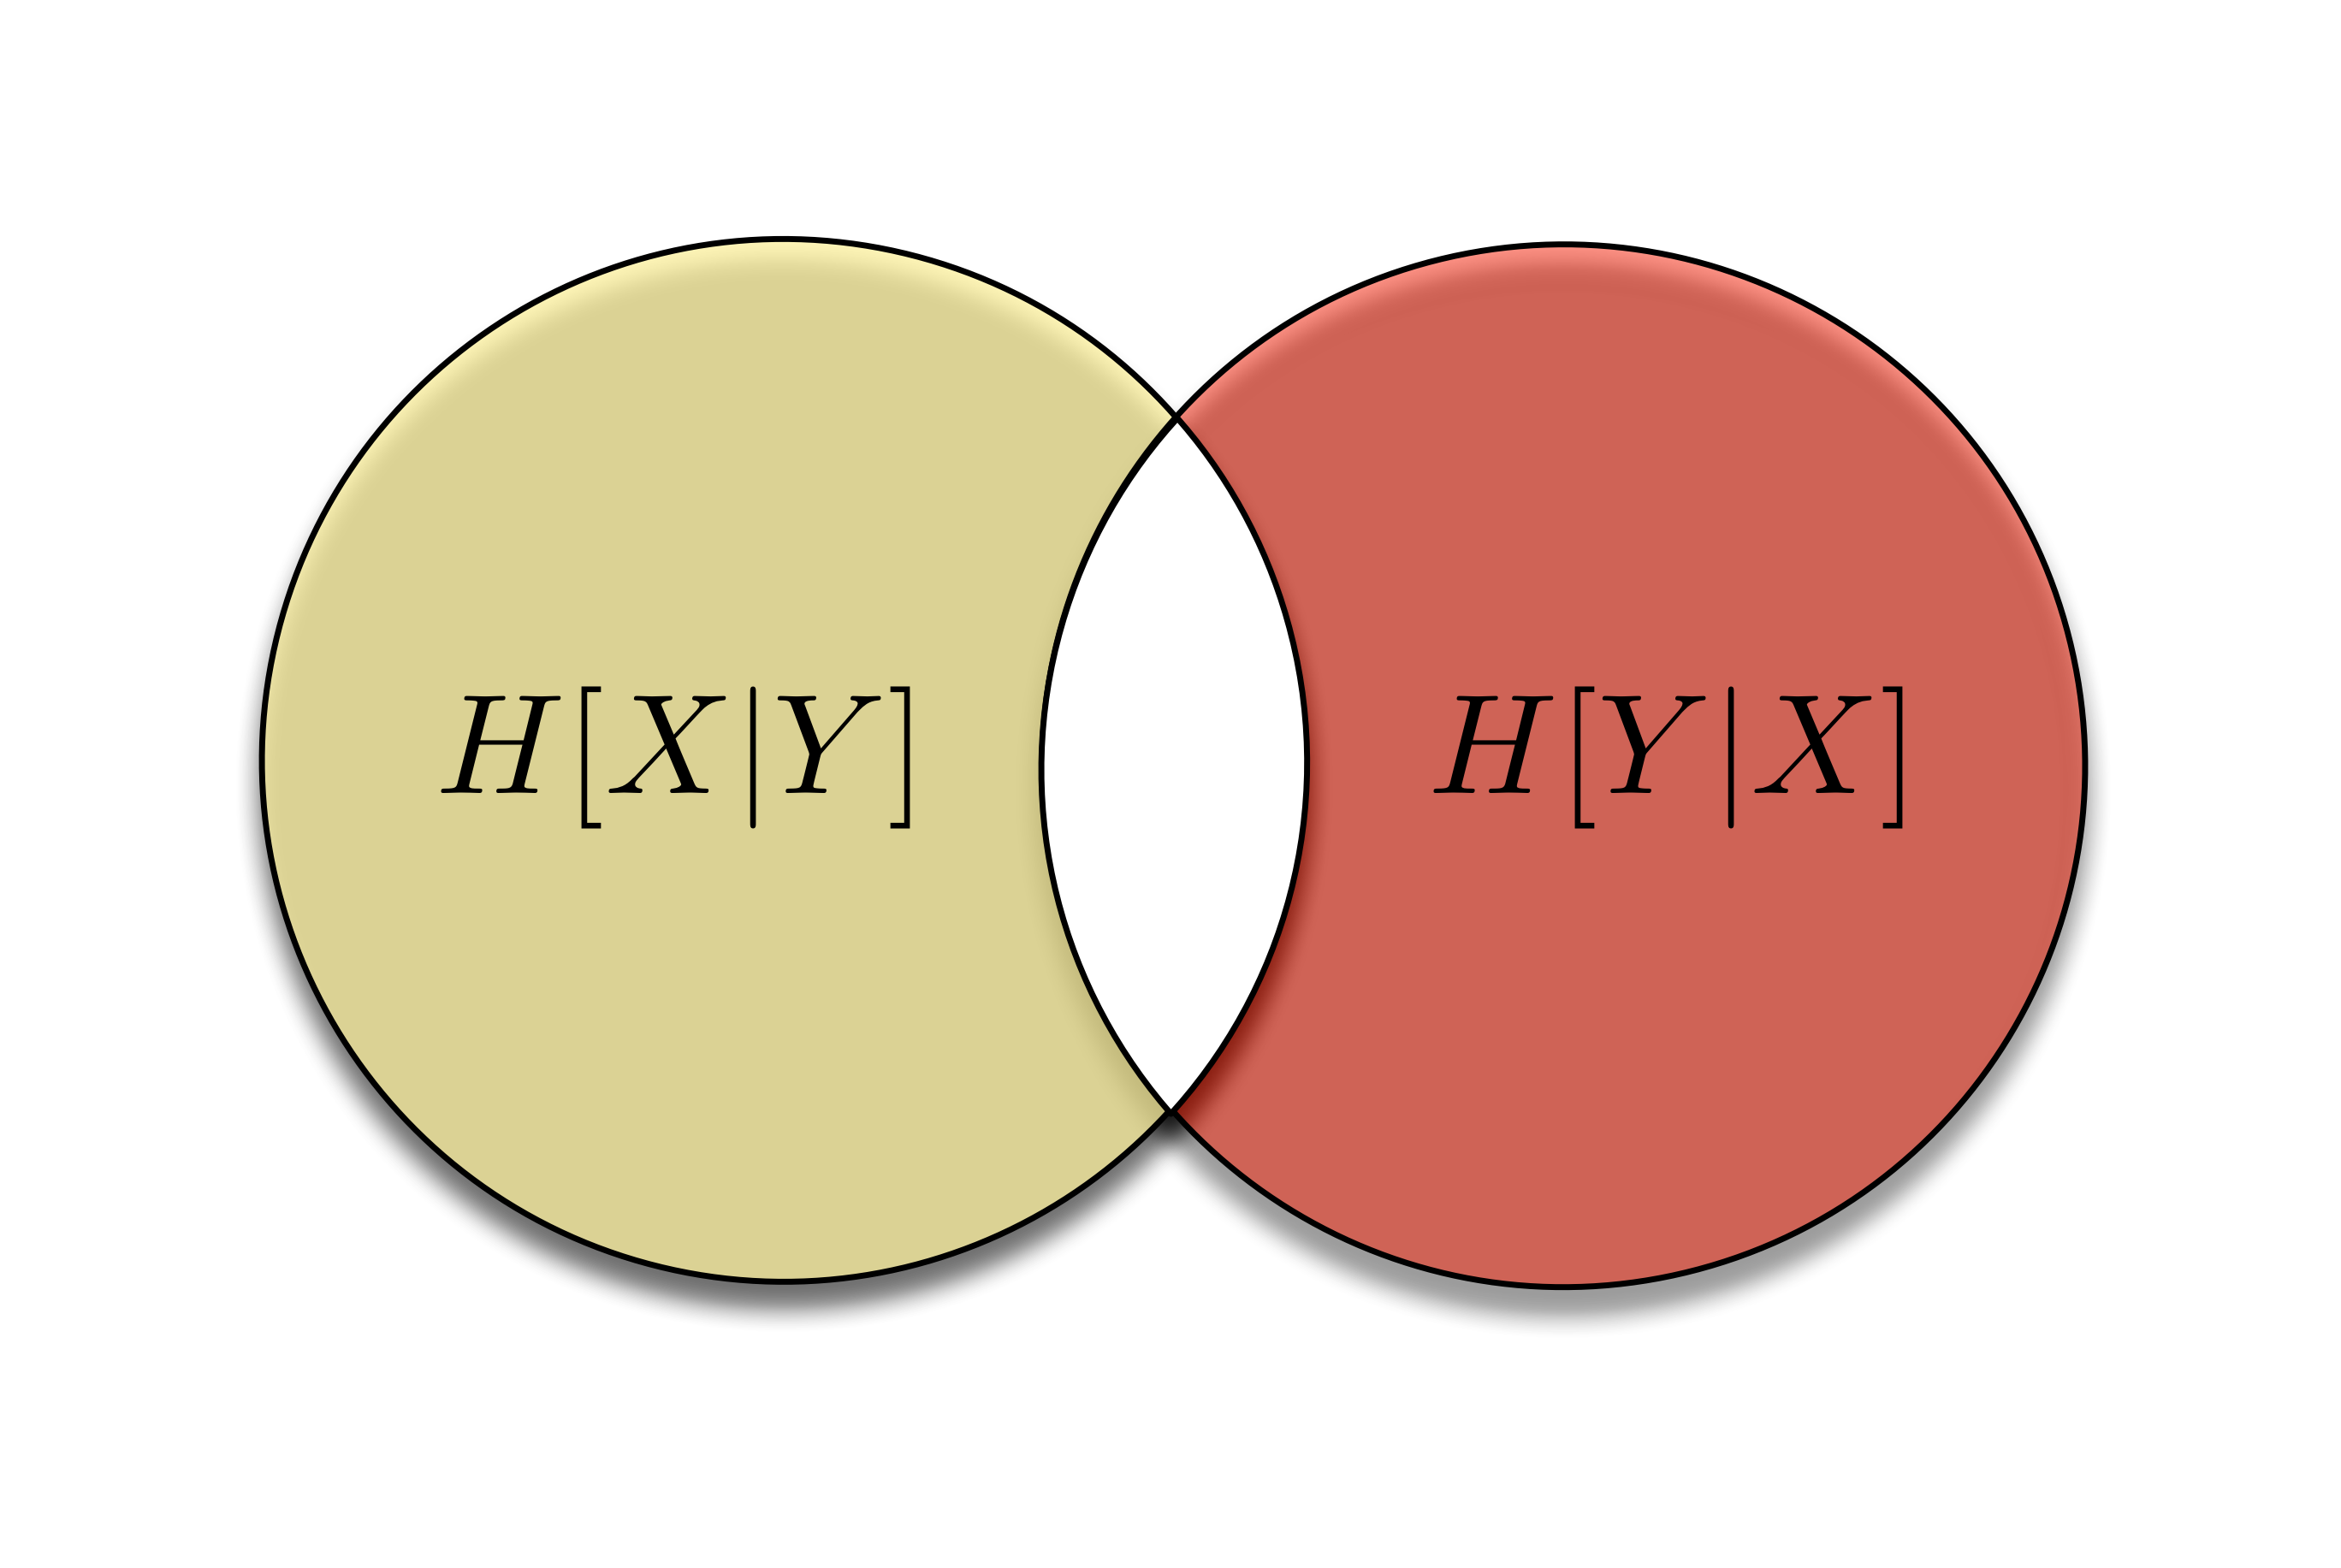
\includegraphics[width=0.50\textwidth]{Figures/Variation-of-Information.png}
\caption{The information diagram representation of variation of information.}
\label{Fig-Information_Diagram}
\end{figure}

For the synthetic example, all but one of the nodes was correctly classified using the weighted community detection algorithm, giving $\text{VI}^{*}[\text{True}; \text{Weighted}] = 0.0115$. In contrast, the variation of information between the unweighted and weighted communities was $\text{VI}^{*}[\text{Unweighted}; \text{Weighted}] = 0.627$. Figure \ref{Fig-Confusion_Matrix_Synthetic} shows the confusion matrix $\mathbf{N}$ for this case. This explains the large variation of information between the two community partitions: the members of the dynamical communities are spread among the `structural' communities identified using the structural network for the synthetic example.

We can perform the same analysis with the Twitter network, but in this case the community partition is unknown. The confusion matrix between the unweighted and weighted community partitions is shown in Figure \ref{Fig-Confusion_Matrix_Twitter}. These partitions give a variation of information of $0.304$. Again, we see from the confusion matrix that the structural communities are generally subdivided amongst the dynamical communities.

\begin{figure}[h!]
  \centering
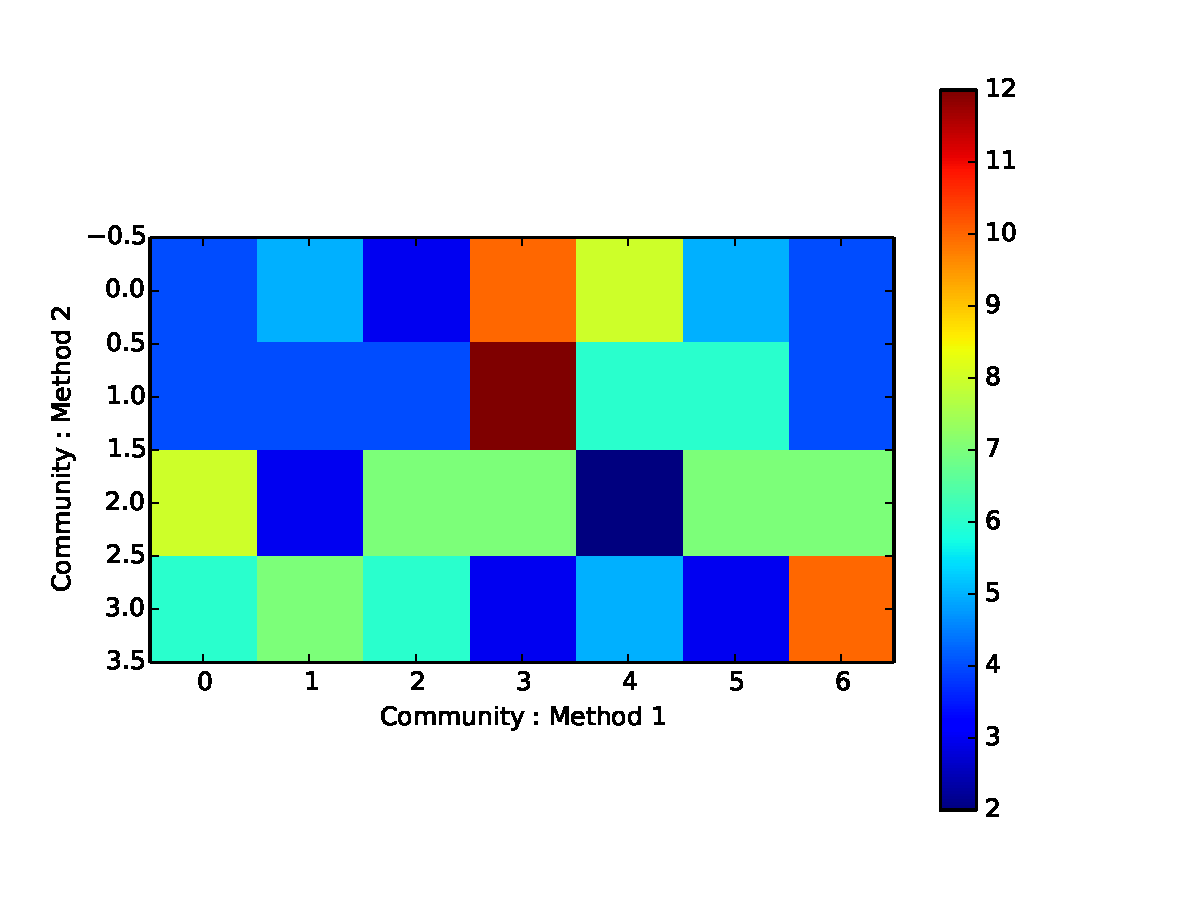
\includegraphics[width=0.75\textwidth]{Figures/confusion_matrix-synthetic.pdf}
\caption{The confusion matrix $\mathbf{N}$ using the communities from the unweighted network (Method 1) and the communities from the weighted network (Method 2) for the synthetic network. The color bar indicates the number of users overlapping between the two partitions.}
\label{Fig-Confusion_Matrix_Synthetic}
\end{figure}

\begin{figure}[h!]
  \centering
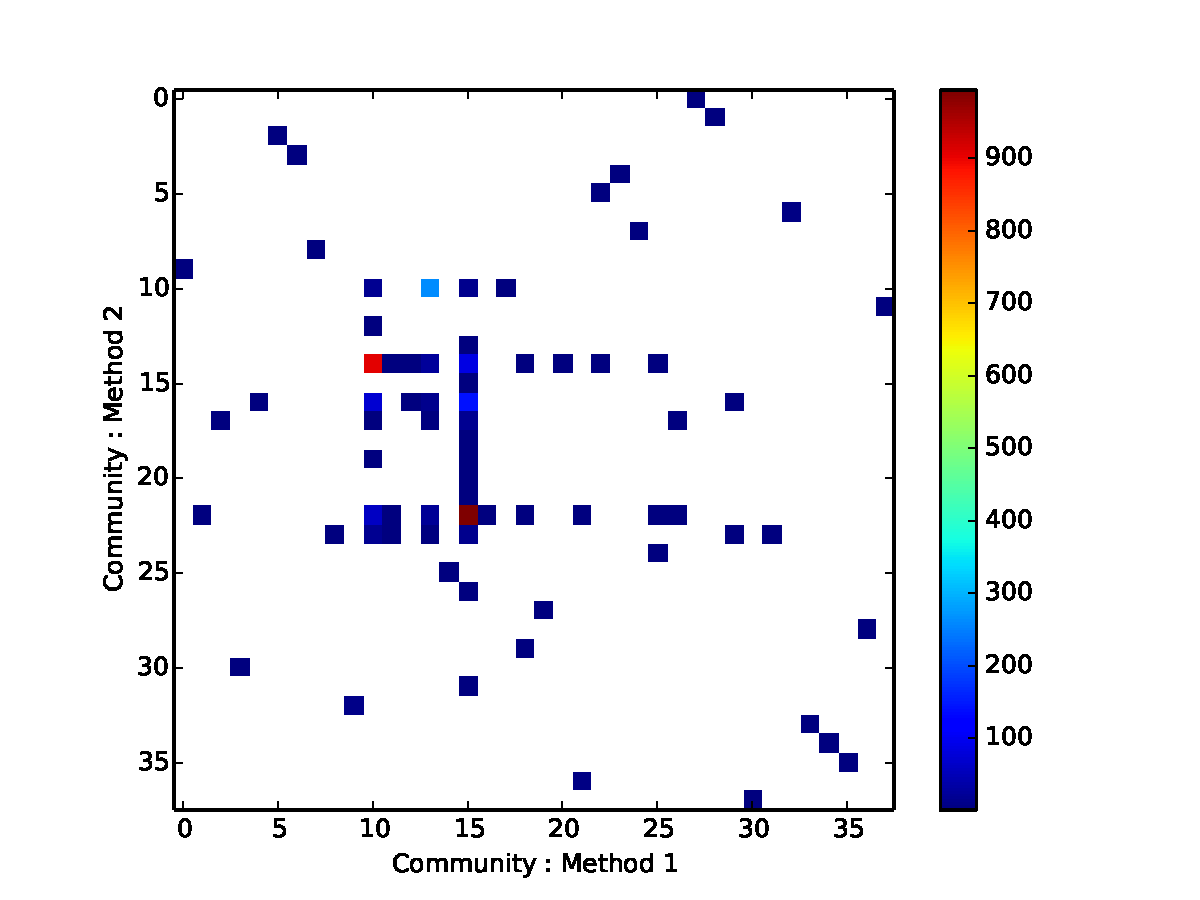
\includegraphics[width=0.75\textwidth]{Figures/confusion_matrix.pdf}
\caption{The confusion matrix $\mathbf{N}$ using the communities from the unweighted network (Method 1) and the communities from the weighted network (Method 2) for the Twitter network. The color bar indicates the number of users overlapping between the two partitions.}
\label{Fig-Confusion_Matrix_Twitter}
\end{figure}

\subsection{Unfolding Structural Communities into Dynamical Communities}\label{sec:unfolding}

As pointed out in~\cite{good2010performance}, due to the limitations of modularity-based community detection, it is important to verify the meaningfulness of communities detected using modularity-based methods. To this end, we considered a particular 236 member \emph{dynamical} community from the Twitter network. This community was chosen because it showed the greatest discrepancy in the normalized mutual information on links internal to the community and links connecting outside the community. That is, for a fixed community, we determined the empirical distribution of the normalized mutual information on the links, conditioned on whether the link is within or without the community. The distance between these two distributions, as measured by the Kolmogorov-Smirnov statistic, gives a notion of how insular the community is. An example of the two conditional empirical distributions is shown in Figure~\ref{Fig-Out_v_In_Links}. As expected given our procedure for determining the dynamical communities, the mutual information on links within the community tended to be much larger than the mutual information on links connecting outside of the community.

\begin{figure}[h!]
  \centering
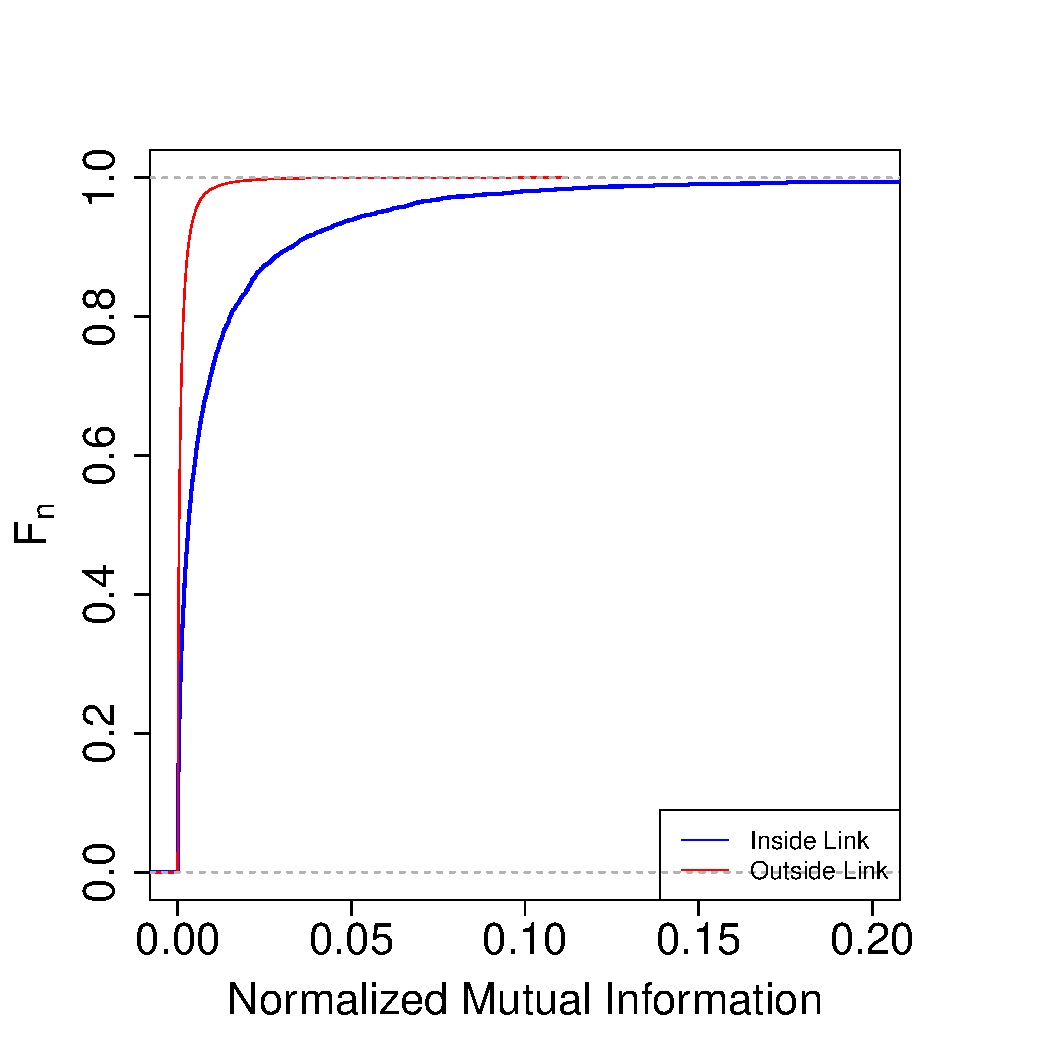
\includegraphics[width=0.50\textwidth]{Figures/out-v-in.pdf}
\caption{The empirical cumulative distribution function for the normalized mutual information on links within (blue) and without (red) a community with 236 members.}
\label{Fig-Out_v_In_Links}
\end{figure}

Because of the large difference in the observed mutual information on the links, we next ranked the internal links for the community based on their associated normalized mutual information. This ranking is shown in Table \ref{Tab-Ranked_nMI}. We see that the vast majority of the high mutual information links correspond to edges between usernames owned by Policy Settlement, a life insurance agency with a Twitter presence. These accounts tended to tweet more or less the same information, staggered slightly in time (within five to ten minutes of each other).

\begin{table}
	\caption{The links with greatest $\hat{I}[X^{u}; X^{v}]$ from a dynamical community with 236 members. The majority of these links belong to Twitter accounts owned by Policy Settlement.}
	\centering
	\begin{tabular}{l l l}
		User $u$ & User $v$ & $\hat{I}^{*}[X^{u}; X^{v}]$ \\ \hline
		LIVEpdq & COImgr & 0.5293023 \\
		RATEpdq & LIVEmgr & 0.5190174 \\
		LIVEpdq & LIVEmgr & 0.4943780 \\
		LIVEpdq & RATEpdq & 0.4892531 \\
		COImgr & LIVEmgr & 0.4820034 \\
		COImgr & RATEpdq & 0.4794285 \\
		LIVEpdq & PolicySettle & 0.4467832 \\
		RATEpdq & PolicyParables & 0.4357249 \\
		PolicySettle & RATEpdq & 0.4276809 \\
		PolicySettle & COImgr & 0.4121432 \\
		COImgr & PolicyParables & 0.3859275 \\
		PolicySettle & LIVEmgr & 0.3843806 \\
		PolicyParables & LIVEmgr & 0.3706989 \\
		PolicySettle & PolicyParables & 0.3565388 \\
		misslindadee & DrAlexConcorde & 0.3557640 \\
		LIVEpdq & PolicyParables & 0.2739896 \\
	\end{tabular}
	\label{Tab-Ranked_nMI}
\end{table}

Moreover, most of the users in this community, like the Policy Settlement accounts, tended to tweet in the very stereotyped ways typical of so-called Twitter bots: user accounts whose posting is controlled by scripts. Thus, this community seems to consist of a large fraction of the Twitter bots amongst the 3000 users, and the large mutual information between the users' dynamics is related to an underlying cause: the scripted tweet behavior.

Other dynamical communities discovered by this approach more closely resemble our intuitions about what community means in social context. For example, the two user community containing the users IntegrativeInfo and JoshuaStarlight are both connected to a Tumblr account run by a single user. Another community of 23 users tended to tweet about technology news. Again, both of these dynamical communities are masked inside the structural communities (1291 and 1086 users, respectively) determined using the unweighted network.

\section{Future Work}\label{sec:futurework}

While our preliminary results are quite promising there are still many things to explore in the future. The first area of research is to better define the notion of \emph{communication} and what we mean by \emph{dynamical community}. Currently we define communication as high mutual information between users in a network. In other words if there exists temporal similarity between two users tweet histories then we say these users are communicating or at least there is information transfer of some kind occurring. This does not however take into account temporally similar but  coincidental tweeting e.g.,  if user $u_1$ and $u_2$ both tweet when they get off work, then these users may be classified as communicating even if they just have similar tweeting schedules and are not actually communicating. On a similar note this ignores users who really do communicate but do so with varying schedules. For example, if $u_1$ tweets during lunch and then $u_2$ retweets $u_1$ at dinner then there is directed communication occurring here and some form of dynamical connectivity even though their tweet histories have low (or no) temporal similarity due to this lag. As a result these users tweet logs would yield very low mutual information and thus we would not categorize them in the same community even if such a community is present.  
By refining our definition of communication to take into account notions such as directionality of information flow and retweet statistics, e.g., weighting a graph by what fraction of retweets come from what users, or trying to measure information transfer through retweet patterns, we may be able to detect different dynamical communities than those detected by our current notion of communication. %Another important piece of data we may be able to utilize about the network is the use of 

%  Another important piece of data we may be able to utilize about the network is the use of retweet statistics, e.g., weighting a graph by what fraction of retweets come from what users, or trying to measure information transfer through retweet patterns.

%This in turn may help bring to surface communities which exist but tweet with varying schedules, e.g., if $u_1$ tweets at lunch and then $u_2$ retweets $u_1$ at dinner then there is directed information transfer occurring here even though they have no temporal connection due to this lag. 





With a refined notion of communication it will become increasingly important to implement information metrics as well as community detection algorithms which adhere to these new standards. For example, on Twitter the act of following someone need not be reciprocated. So there is a natural direction to structural edges in the network, the community detection algorithms we utilized as well as the information measure we used (i.e. normalized-mutual information) are all non-directional. If we instead used a directed information measure such as transfer entropy~\cite{schreiber2000measuring} along with a community detection algorithm which worked on directed graphs we may be able to see new and interesting dynamical networks, which were not present by merely ignoring this natural direction of the network. 



In addition to deeper analysis of what communication really is and the ramifications this will have on our methods, it is also important to analyze the validity of community detection based on modularity maximization as discussed in~\cite{good2010performance}. Other possibilities would be using community detection which do not rely on modularity e.g., Infomap \cite{Rosvall08mapsof} or weighted stochastic block models~\cite{aicher2013adapting}. 

With a strong definition of communication, information measures and true \emph{dynamical}-community detection algorithms to bring to life this definition, we should be able to bring to light which users belong to which dynamical  communities. What these actual communities are and why they exist however will require a more ``sociological" touch. Once dynamical communities are detected we hope to analyze the tweet content more extensively either through natural language processing techniques or by hand.  As was done with the Twitter-bot analysis in Section \ref{sec:unfolding}.

%Finally we need to do a more in depth literary review, communication detection and network analysis of Twitter data is a vast set of work and we need to really explore what has already been done to see what future directions to take this work. 

% as when the people tweet but we have to consider if this is the most accurate measure of communication. With this question answered exploring more interesting detection algorithms will be possible such as.... 

% So far we considered a normalized measure of mutual information. 
% Should we explore other kind of information flow measures?


%- What about tracking information flow through retweets?

%- So far we used two communities detection algorithms (Leuven [1] and the one used by Cesar), but there are many more and we should probably test a few of them
%- Discussion about �static network + dynamics on the network� vs �network whose structure also evolves over time�
%- Investigate the structure and the dynamics of the Twitter communities with a more �sociological� approach, to try to characterize them and see if they have different behaviours
%- We need a deeper literature review!

 %Q for meeting... 
% 1. what types of information flow should we apply? transfer entropy as opposed to mutual information and then expanding the discussion to directed graphs which is probably more appropriate for twitter data with community detection on directed graphs. 
 
% Better definition for communication. currently the definition is mutual information between when people tweet. 
 
% Do a weighted graph by fraction of retweets by a user. So looking at fraction of retweets for a particular user, so using the information of the tweets 
 
% this might pick up log term lag stuff or compute mutual information over lags. 
 
% 2. Can we track information flow through retweets with the new retweet engine?
%maybe because we have old data
%
%3. What other detection algorithms would be useful, 
%for static network we have Blondel et al. (which is the modularity one) and then we use the one with weighting using mutual information (citation), do we use others ... 

%then for nonstatic analysis. It seems like the discussion of detection with time snapshots implies the network structure is actually changing too and for this we use Kawadia and Screenivasan algorithm but then there is Mucha for layered detection ... does this fall into static?


%We use optimization of modulatory, may also be useful to use other such as stochastic block model or info map. 

%4.Investigate the structure and the dynamics of the Twitter communities with a more �sociological� approach, to try to characterize them and see if they have different behaviors.... 
%So now actually examine the communities by hand and see if the communities match...Can you then use an information measure to gather statistics on twitter usage e.g., when people tweet in various communities. 




%5. -We currently do a  �static network + dynamics on the network� should we dicuss a  �network whose structure also evolves over time� maybe how that network grows with respect to information transfer?

%7. finally a deeper lit review

\section{Conclussions}\label{sec:conclusions}

In this paper we have researched two networks that represent systems of social interactions: one
was derived from a toy model and the other was reconstructed from Twitter, a microblogging service
whose network is provided by users \emph{following} each other. We have shown that a weighting of the
links with the mutual information between any two connected nodes might provide a refinement of
the network, and that this refinement brings us closer to the underlying constituents of the
networks. We note that the toy model was generated with specified number of
communities, where community membership determines the activity of each node as a
consequence of the activity of the others. In the real-world network the number of communities -- if
any -- is unknown.

    We searched for community structure using both the unweighted and weighted adjacency matrices, using an
algorithm whose performance has been assessed by other authors and that is adequate to deal
with a great number of nodes. In the toy model, the community structure determined using only the unweighted network is fragmented
and differs from the one known by construction. Meanwhile, using the weighted
network faithfully recovers the structure that we had imposed. In the case of Twitter users, the
communities detected in the unweighted network appear less fragmented than the ones we recover after
weighting the links. Both weighted networks feature a higher optimal modularity than their
unweighted counterparts. This result suggests that the clusters detected in the weighted version are
more likely to constitute actual communities, as we know that is the case in the toy model. We
assessed a singular cluster from the Twitter network, finding that it seems driven by bots posting
on behalf of a life insurance company.

    Coming back to the very important questions posed during the introduction, we should acknowledge
the difficulty in them before claiming any definitive resolution. Both in the toy model and the Twitter case the constituents were brought
together to perform a social interaction, either real or simulated. We have a first approach that
provides clear-cut networks with all or nothing links, and a second one weighting the links somehow
based on the social activity, which is the very reason--we argue--why the networks came into
existence in the first place. Based on the results, we can only reconstruct the known structure of
the toy model after these interactions have been taken into account. If we extend the reliability of
these results to the real world network, weighting the links based on the activity
of the nodes reveals the object under research in a deeper, more informative manner.

\bibliographystyle{plain}
\bibliography{references}

\end{document}